\chapter{Experiment Results}\label{ch:exp-result}
This appendix provides supplementary figures and tables supporting the results presented in Section \ref{sec:experiment-results} and analysed in Section \ref{sec:exp-analysis-interpretation}. Section \ref{sec:exp-general-overview} presents an overview of the category scores across all experiments, broken down by grid size and individual metric. Section \ref{sec:exp-stress-test} shows the total score distributions for each of the three stress test experiments. Section \ref{sec:exp-single-scenario} provides a detailed, run-level breakdown of the category scores for every scenario of the standard, diverse and stress test experiments. Finally, Section \ref{sec:exp-case-study} illustrates the partial grid topologies resulting from the \ac{ppo} agent's actions in the three case studies discussed in Section \ref{ssec:case-studies}.


\section{General Overview}\label{sec:exp-general-overview}
This section presents a condensed overview of the results across all experiments, first as a heatmap over all scenarios, then broken down by grid size, and finally by individual metric.

\subsection{Scenario Heatmap}
Figure \ref{fig:exp-heatmap} gives a condensed overview of the category scores achieved by the three evaluated agents across all experiments, grouped by grid size.

\begin{figure}[htp] % htp = hier (h), top (t), oder auf einer eigenen Seite (p).
    \centering
    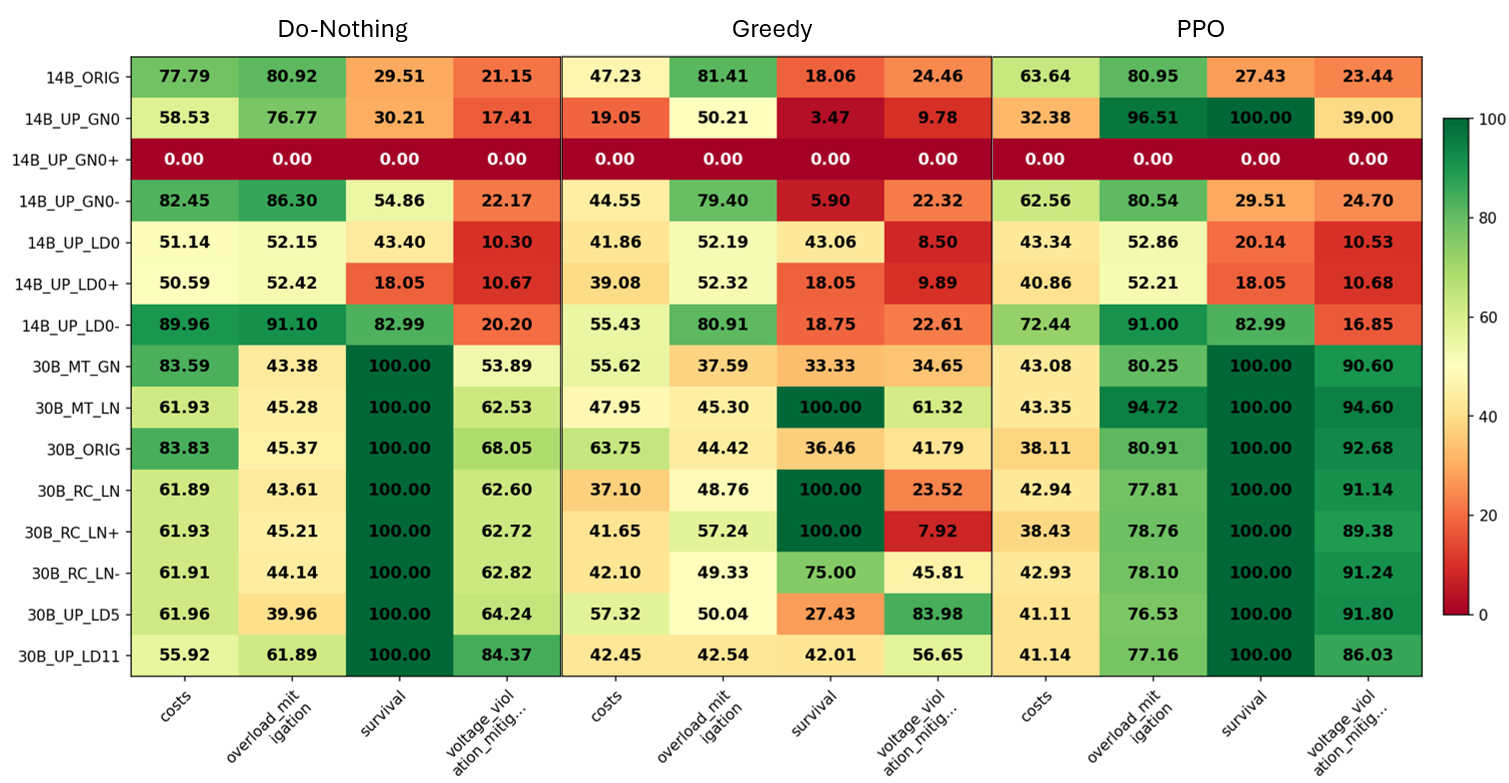
\includegraphics[width=1\textwidth]{images/experiments/heatpmap.png}
    \caption{Category score heatmaps over all experiments for the three evaluated agents}
    \label{fig:exp-heatmap} 
\end{figure}

\FloatBarrier

\subsection{Bus Comparison}
Figure \ref{fig:bus-scores} compares the category scores of the three agents between the 14-bus and 30-bus power grids, highlighting differences in agent performance depending on grid size.

\begin{figure}[htp] % htp = hier (h), top (t), oder auf einer eigenen Seite (p).
    \centering
    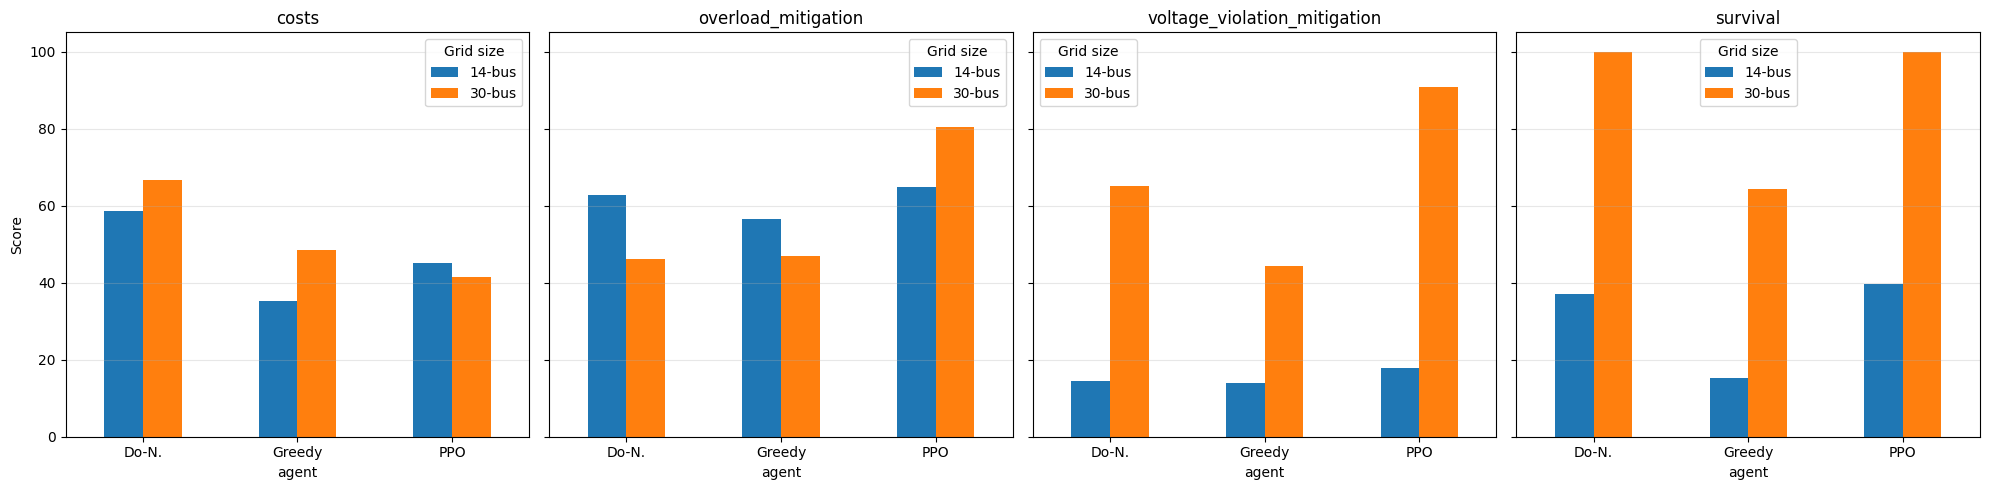
\includegraphics[width=1\textwidth]{images/experiments/bus_scores.png}
    \caption{Category score between the 14- and 30-bus power grids}
    \label{fig:bus-scores} 
\end{figure}


\subsection{Metric Comparison}
Figure \ref{fig:metric-scores} breaks down the category scores of Figure \ref{fig:exp-heatmap} further into their individual metrics, shown separately for the cost, overload mitigation, survival, and voltage violation mitigation categories.

\begin{figure}[htp]
    \centering
    \begin{subfigure}[t]{1\textwidth}
        \centering
        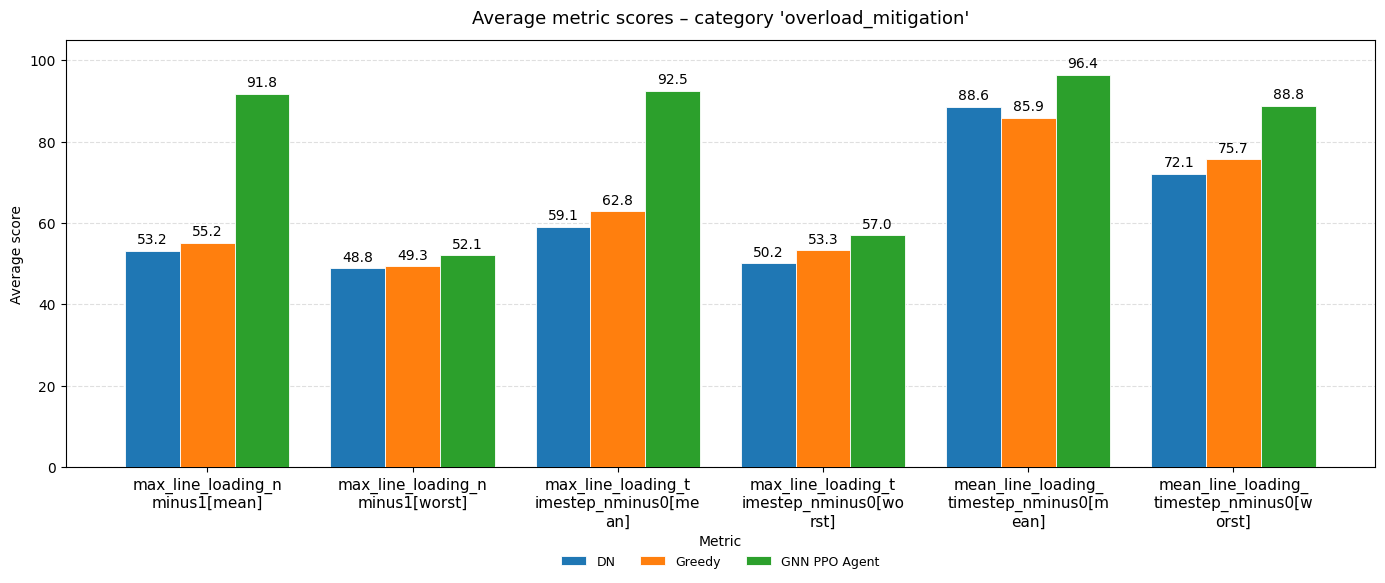
\includegraphics[width=0.9\textwidth]{images/experiments/metric_scores/overload_mitigation1.png}\\[0.1em]
        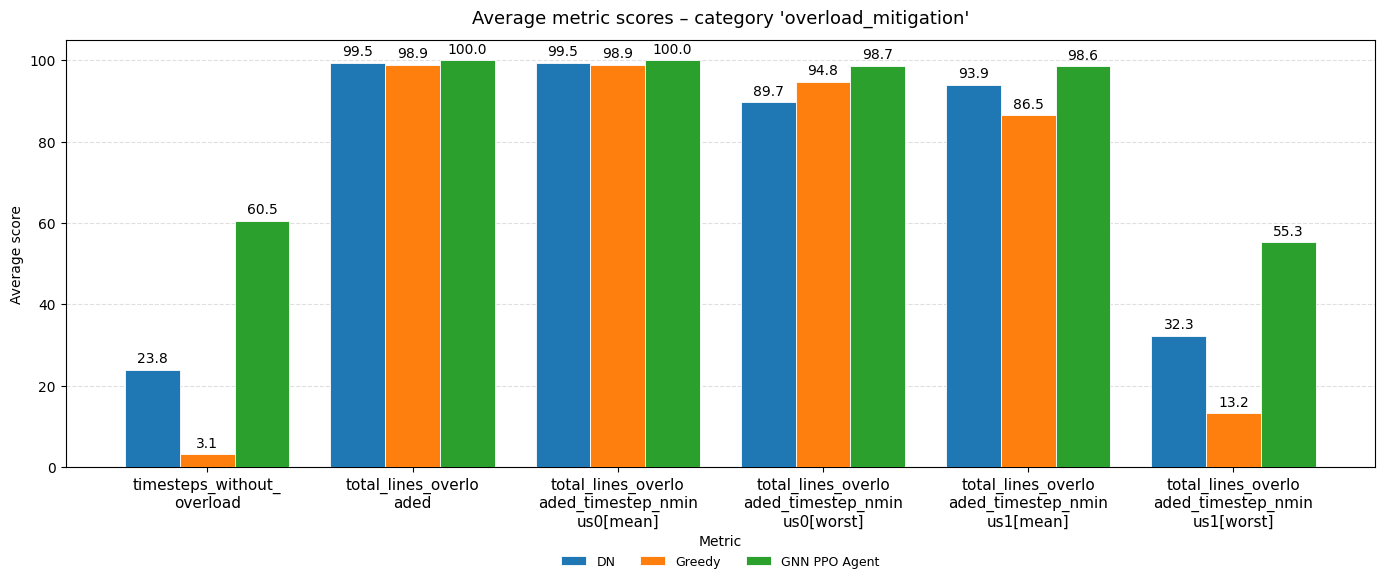
\includegraphics[width=0.9\textwidth]{images/experiments/metric_scores/overload_mitigation2.png}
        \caption{Metric scores over the overload mitigation category for the three evaluated agents}
        \label{fig:metric-scores-overload} 
    \end{subfigure}
    \caption{Metric scores over different categories for all three evaluated agents}
    \label{fig:metric-scores}
\end{figure}

\begin{figure}[htp]
    \ContinuedFloat
    \centering

    \begin{subfigure}[t]{1\textwidth}
        \centering
        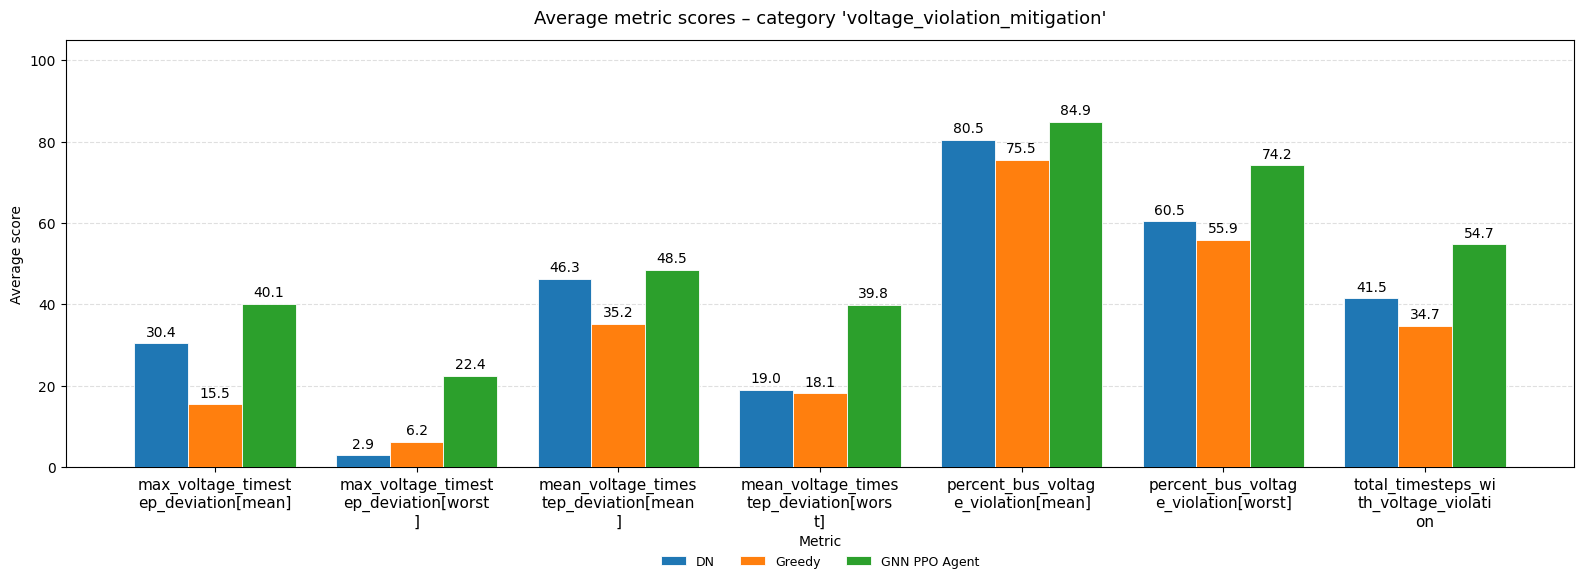
\includegraphics[width=\textwidth]{images/experiments/metric_scores/voltage_violation_mitigation.png}
        \caption{Metric scores over the voltage violation mitigation category for the three evaluated agents}
        \label{fig:metric-scores-voltage-violation} 
    \end{subfigure}

    \vspace{0.2em}

    \begin{subfigure}[t]{1\textwidth}
        \centering
        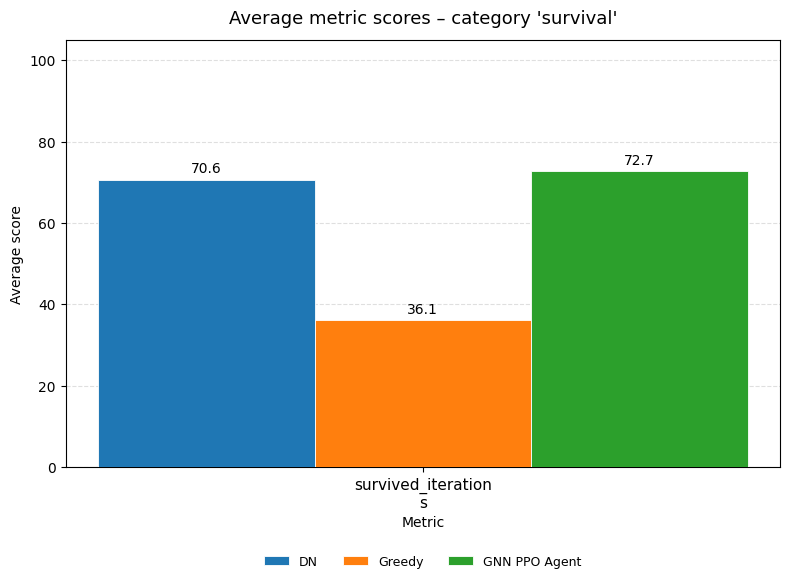
\includegraphics[width=0.55\textwidth]{images/experiments/metric_scores/survival.png}
        \caption{Metric scores over the survival category for the three evaluated agents}
        \label{fig:metric-scores-survival} 
    \end{subfigure}

    \vspace{0.2em}

    \begin{subfigure}[t]{1\textwidth}
        \centering
        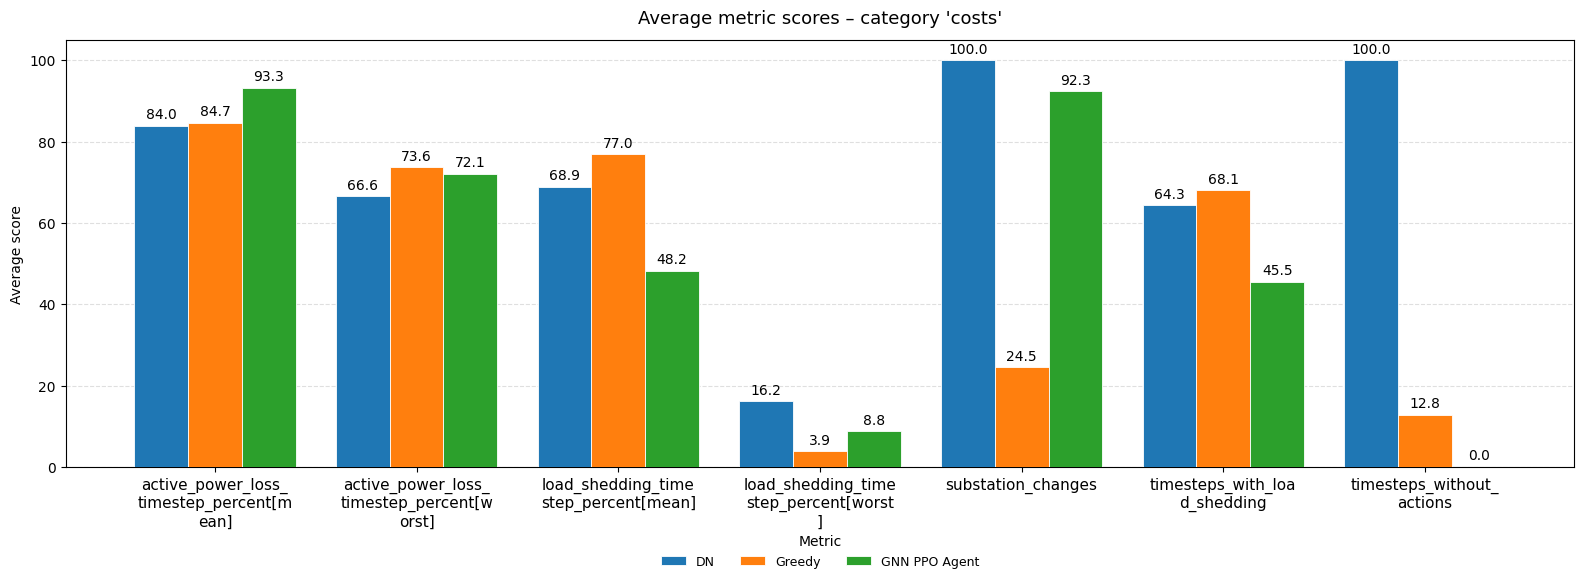
\includegraphics[width=\textwidth]{images/experiments/metric_scores/costs.png}
        \caption{Metric scores over the cost category for the three evaluated agents}
        \label{fig:metric-scores-costs} 
    \end{subfigure}

    \caption{Metric scores over different categories for all three evaluated agents (continued)}
\end{figure}

\FloatBarrier







\section{Stress Test}\label{sec:exp-stress-test}
Figures \ref{fig:tot-score-gen-stress}, \ref{fig:tot-score-load-stress}, and \ref{fig:tot-score-line-cap-stress} show the total score distributions achieved by the three agents across the increasing stress levels of the generator, load, and line capacity stress test experiments, respectively.

\begin{figure}[htp] % htp = hier (h), top (t), oder auf einer eigenen Seite (p).
    \centering
    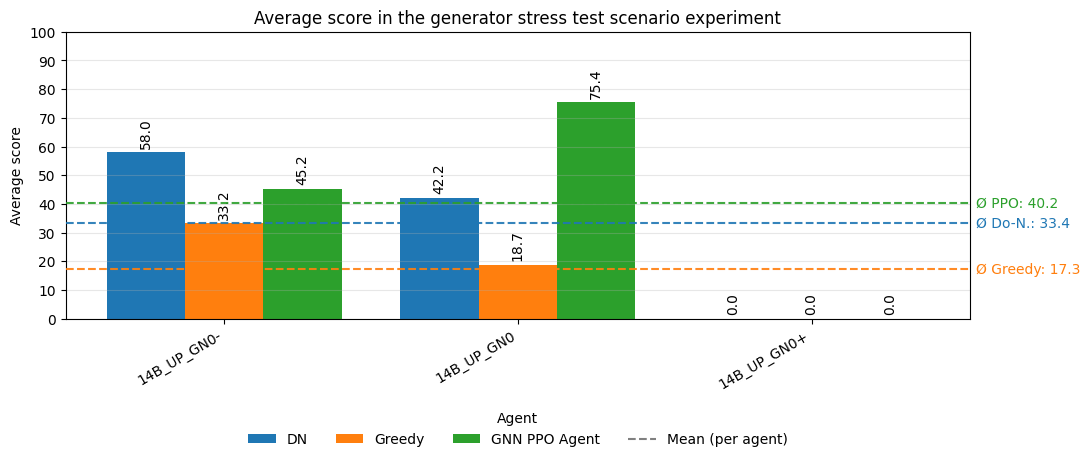
\includegraphics[width=0.87\textwidth]{images/experiments/total_scores/gen_stress.png}
    \caption{Total score overview for the generator stress test experiment, with average values of each agent}
    \label{fig:tot-score-gen-stress} 
\end{figure}


\begin{figure}[htp] % htp = hier (h), top (t), oder auf einer eigenen Seite (p).
    \centering
    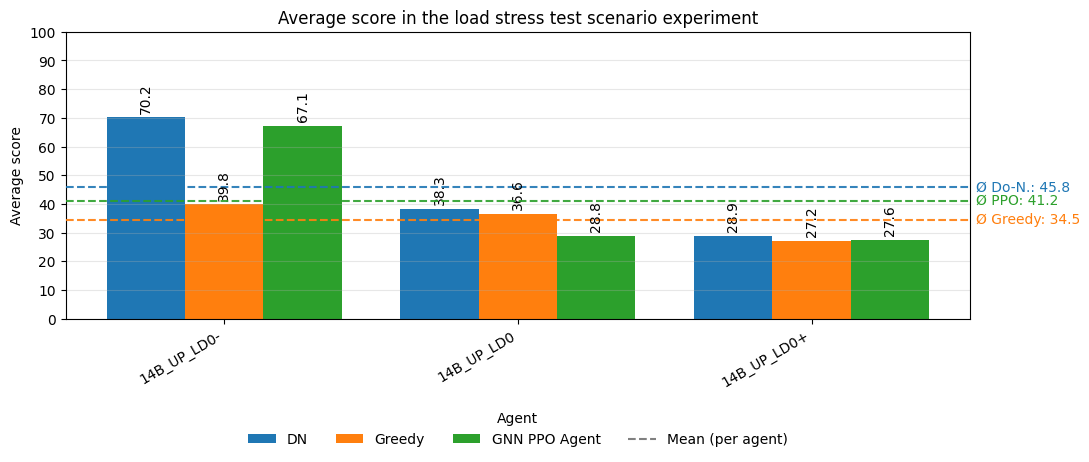
\includegraphics[width=0.87\textwidth]{images/experiments/total_scores/load_stress.png}
    \caption{Total score overview for the load stress test experiment, with average values of each agent}
    \label{fig:tot-score-load-stress} 
\end{figure}


\begin{figure}[htp] % htp = hier (h), top (t), oder auf einer eigenen Seite (p).
    \centering
    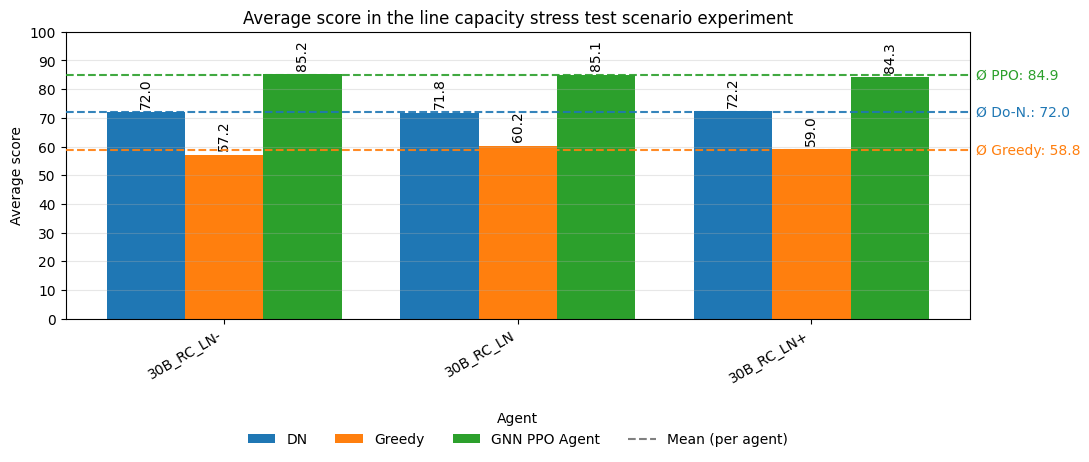
\includegraphics[width=0.87\textwidth]{images/experiments/total_scores/line_cap_stress.png}
    \caption{Total score overview for the line capacity stress test experiment, with average values of each agent}
    \label{fig:tot-score-line-cap-stress} 
\end{figure}

\FloatBarrier





\section{Single Scenario Comparison}\label{sec:exp-single-scenario}
This section provides a detailed, run-level breakdown of the category scores for every scenario evaluated in the standard, diverse and stress test experiments, complementing the aggregated results shown in Sections \ref{sec:exp-general-overview} and \ref{sec:exp-stress-test}.

\subsection{Standard Test Scenarios}
Figure \ref{fig:scenario-scores-orig} shows the category scores achieved by the three agents on the two unmodified base grids.

\begin{figure}[htp]
    \centering
    \begin{subfigure}[t]{1\textwidth}
        \centering
        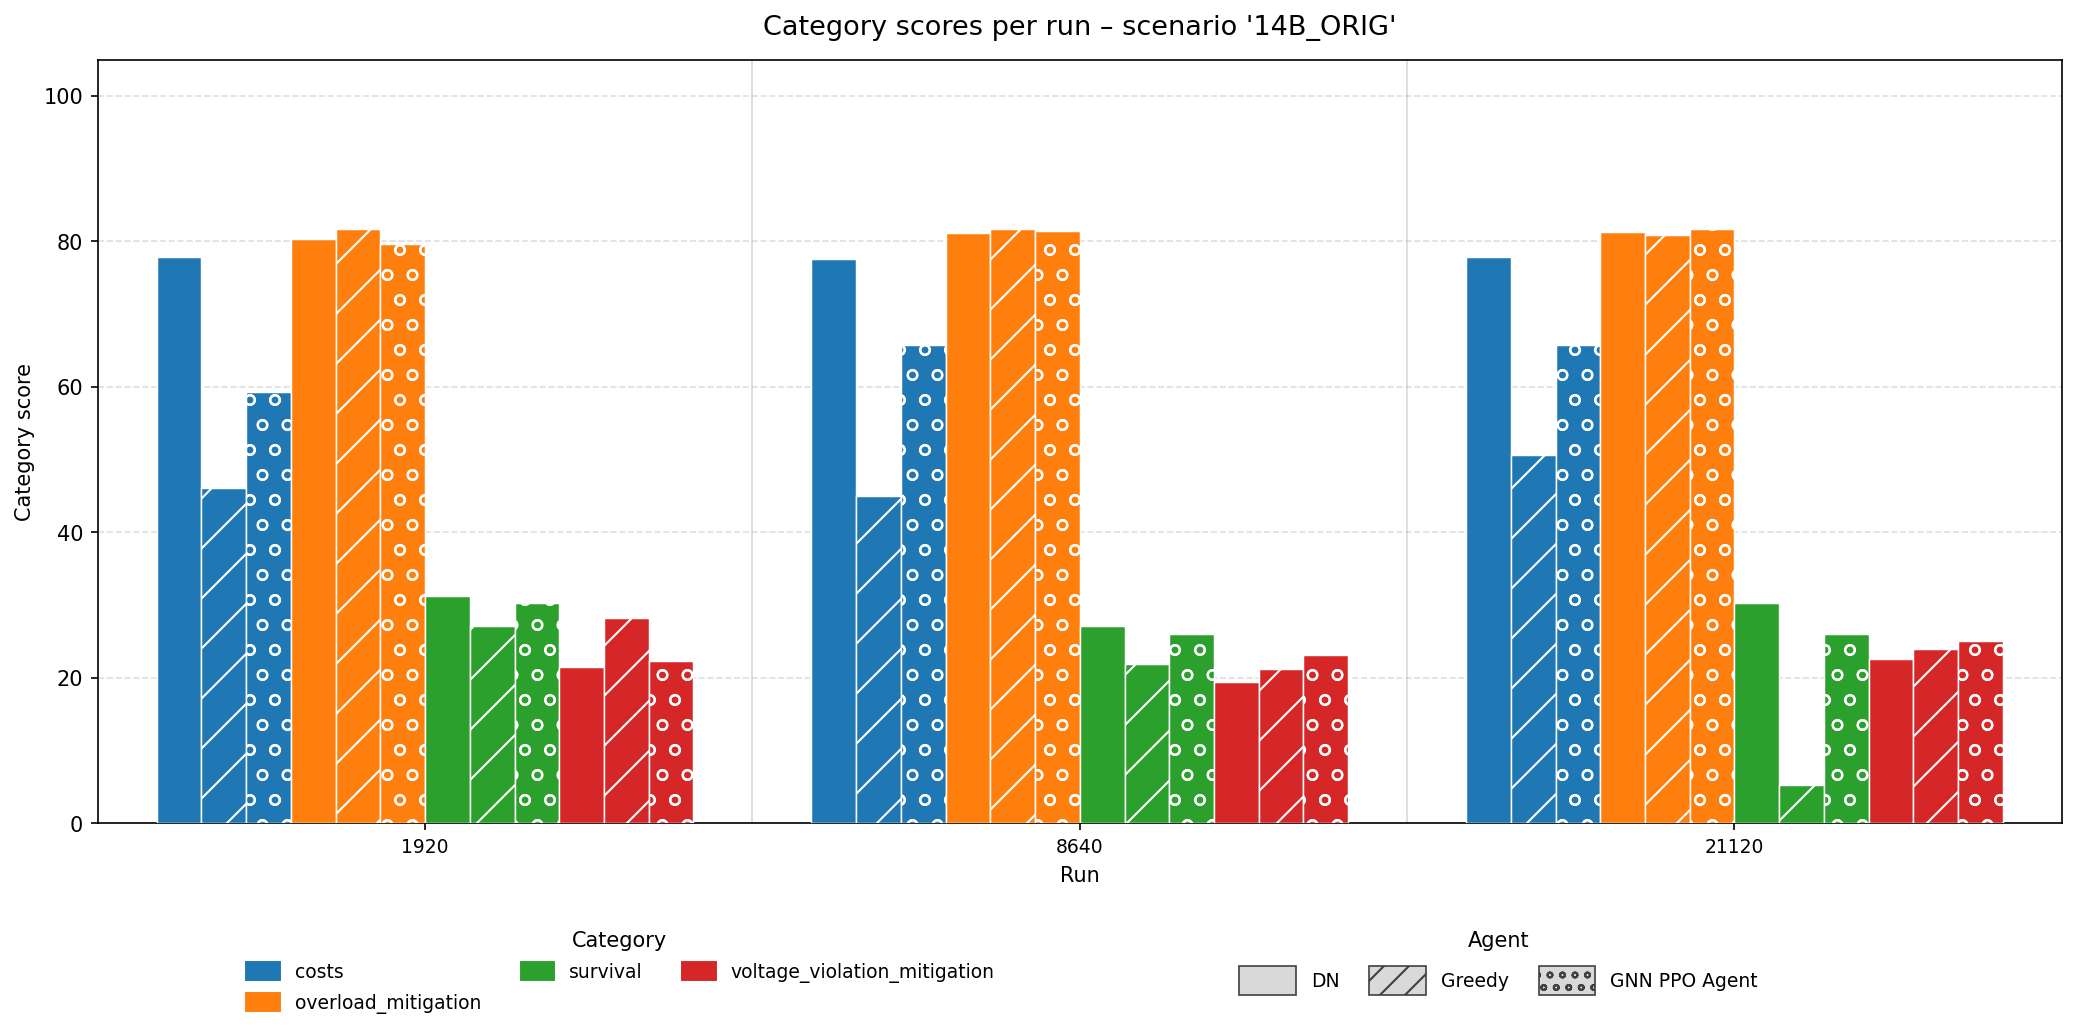
\includegraphics[width=\textwidth]{images/experiments/scenario_scores/14B_ORIG.png}
        \caption{14-bus unmodified power grid}
        \label{fig:scenario-scores-14b-orig}
    \end{subfigure}

    \vspace{0.2em}

    \begin{subfigure}[t]{0.65\textwidth}
        \centering
        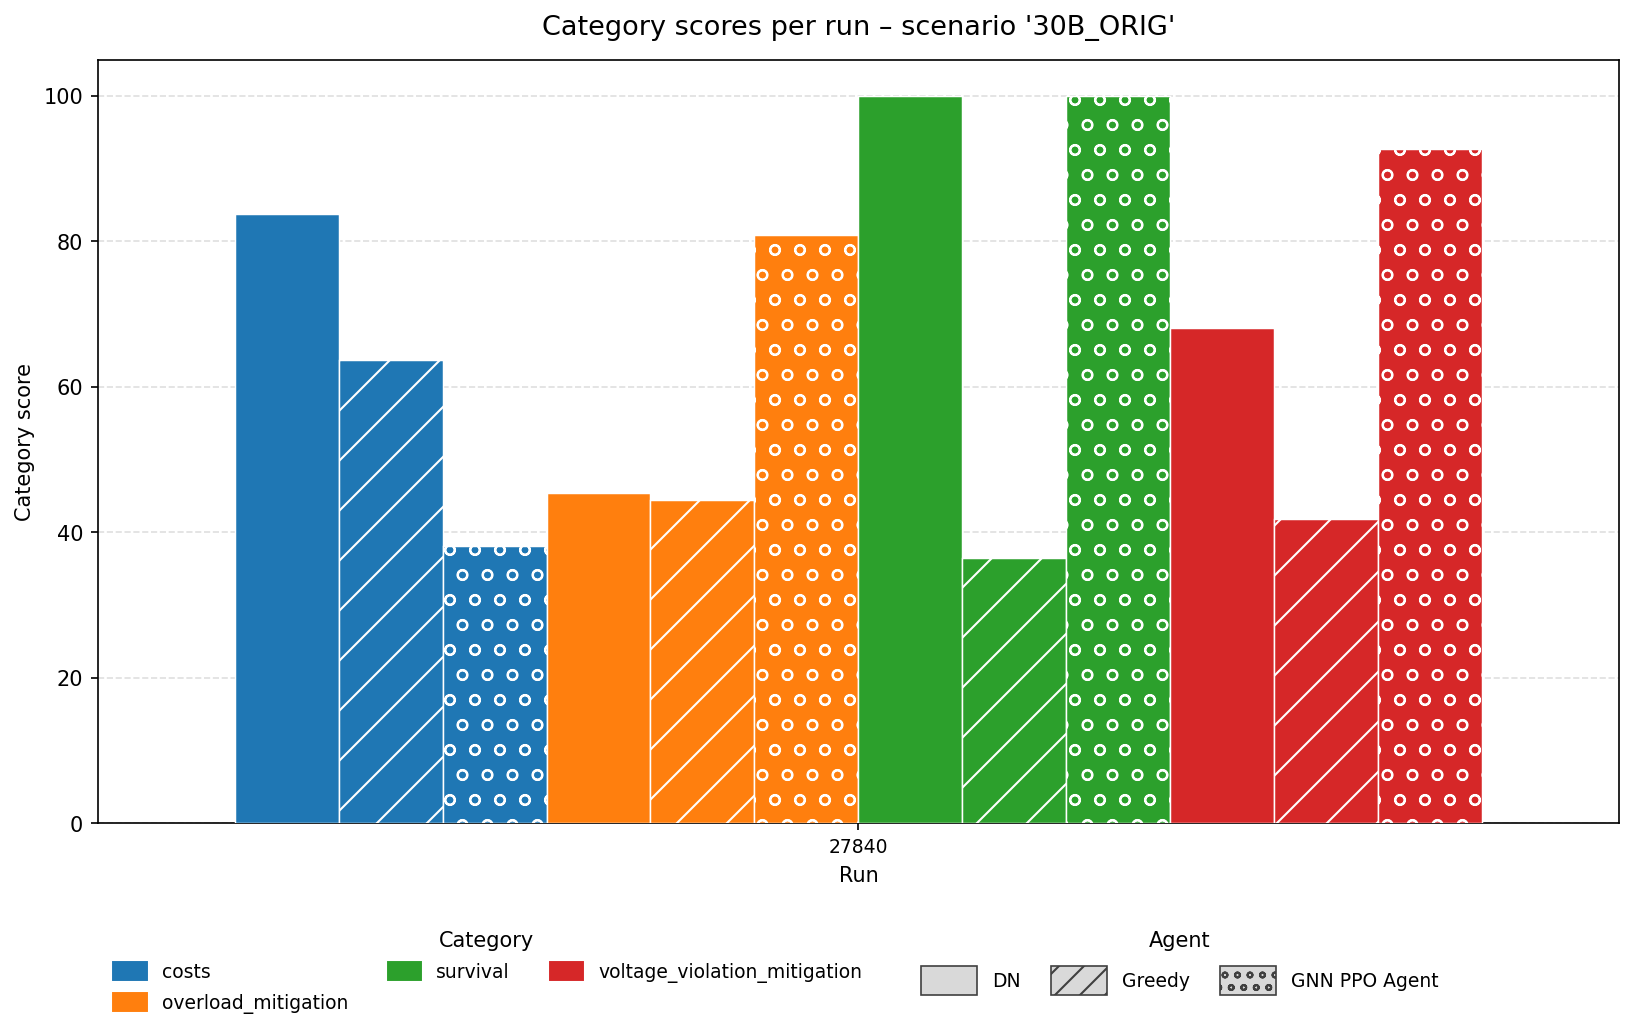
\includegraphics[width=\textwidth]{images/experiments/scenario_scores/30B_ORIG.png}
        \caption{30-bus unmodified power grid}
        \label{fig:scenario-scores-30b-orig}
    \end{subfigure}

    \caption{Score overview over the standard test runs}
    \label{fig:scenario-scores-orig}
\end{figure}

\FloatBarrier

\subsection{Diverse Scenarios}
Figures \ref{fig:scenario-scores-14b-gnld-scaled} to \ref{fig:scenario-scores-rc} show the category scores achieved by the three agents on the diverse scenarios, in which either a generator or load was scaled, a maintenance event was triggered, or the thermal line capacity was reduced.

\begin{figure}[htp]
    \centering

    \begin{subfigure}[t]{1\textwidth}
        \centering
        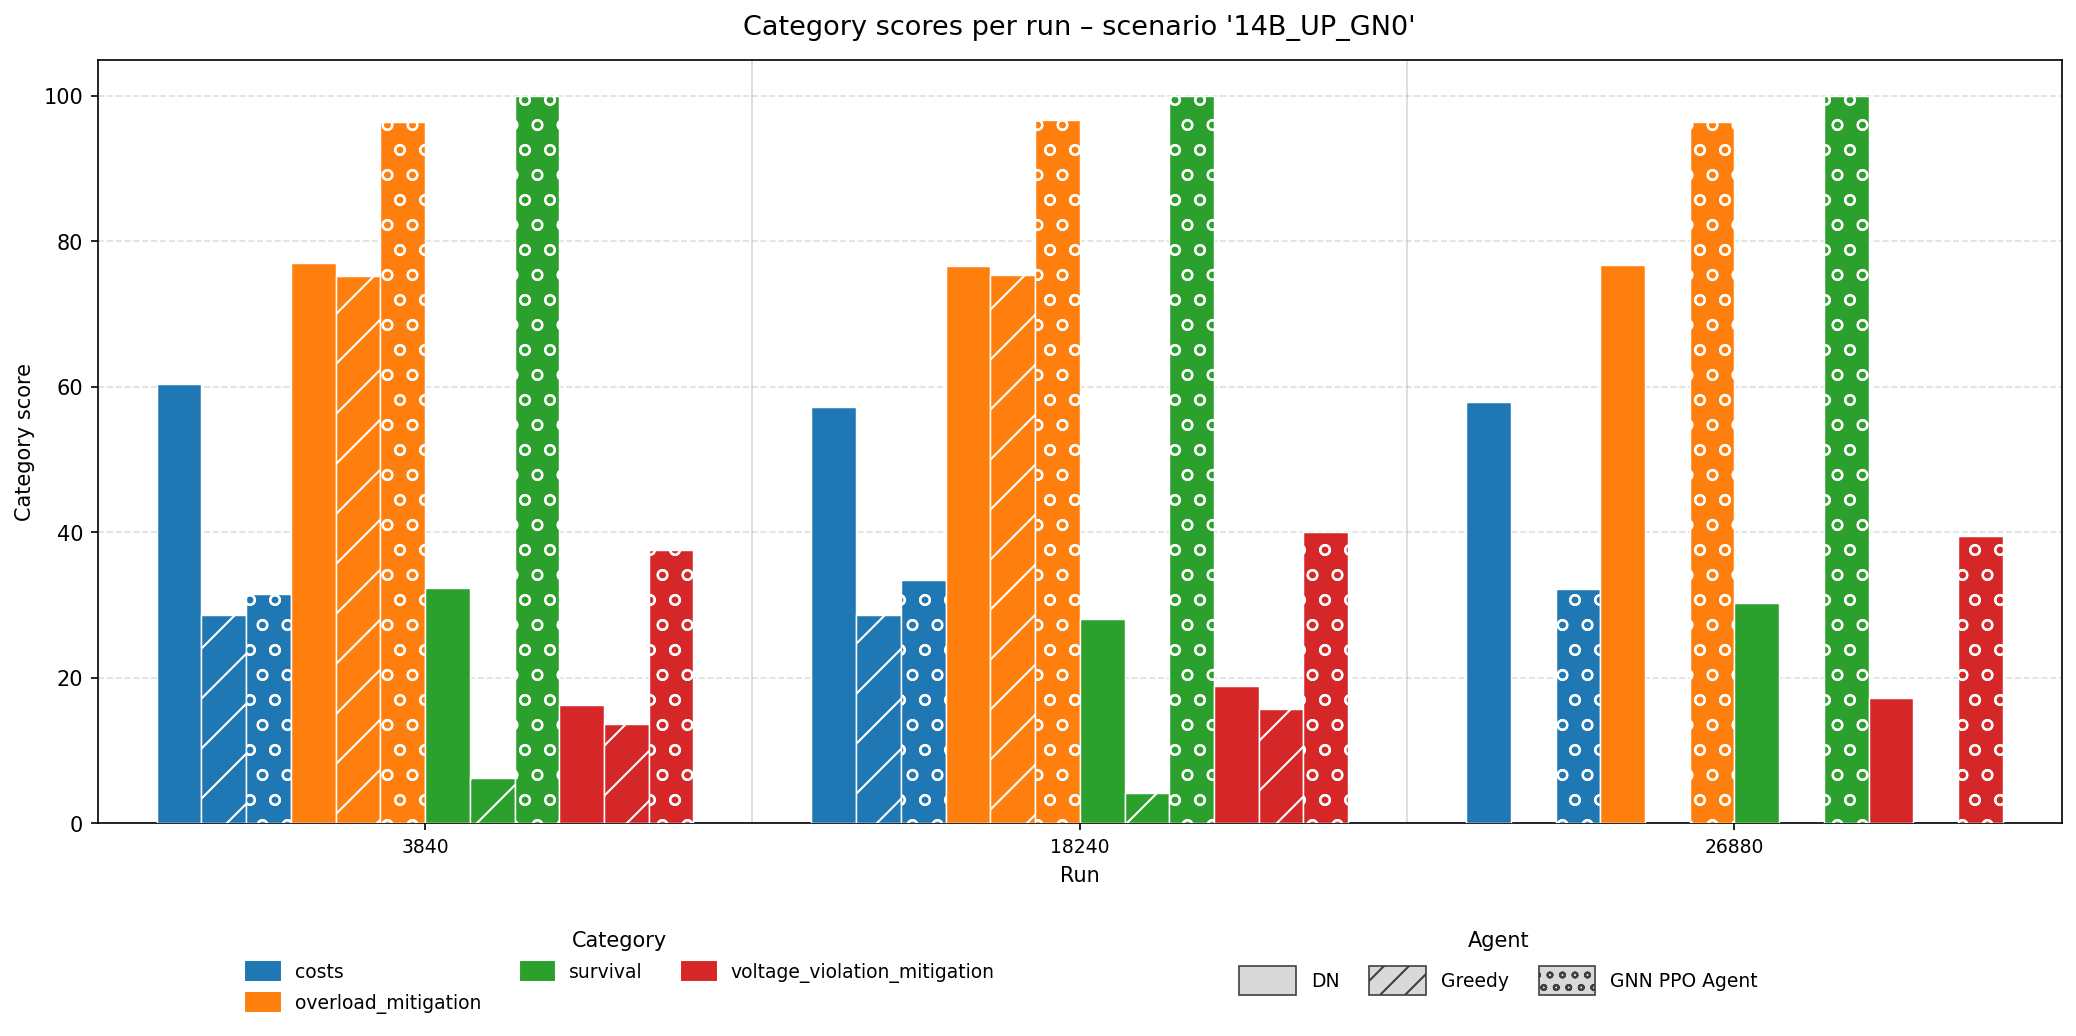
\includegraphics[width=\textwidth]{images/experiments/scenario_scores/14B_UP_GN0.png}
        \caption{14-bus with increased power generation in generator 0}
        \label{fig:scenario-scores-14b-up-gn0} 
    \end{subfigure}

    \vspace{0.2em}

    \begin{subfigure}[t]{0.65\textwidth}
        \centering
        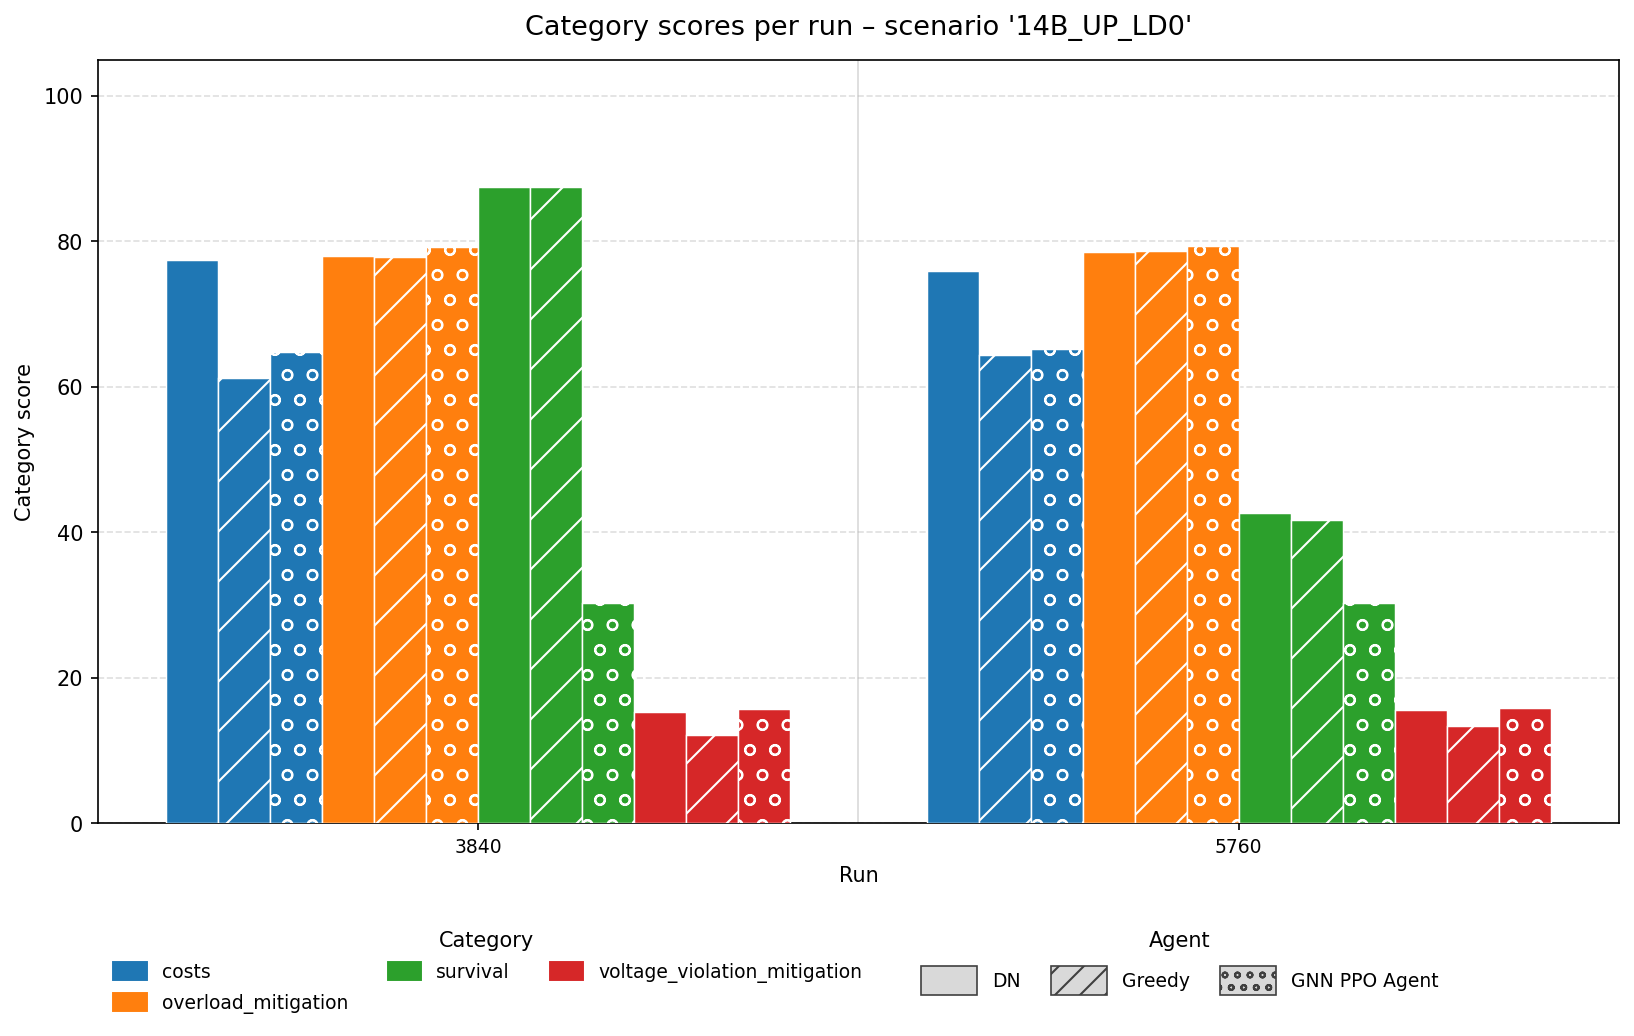
\includegraphics[width=\textwidth]{images/experiments/scenario_scores/14B_UP_LD0.png}
        \caption{14-bus with increased power consumption in load 0}
        \label{fig:scenario-scores-14b-up-ld0}
    \end{subfigure}

    \caption{Score overview over the scenarios in the 14-bus grid in which a generator or load was modified}
    \label{fig:scenario-scores-14b-gnld-scaled}
\end{figure}

\begin{figure}[htp]
    \centering

    \begin{subfigure}[t]{1\textwidth}
        \centering
        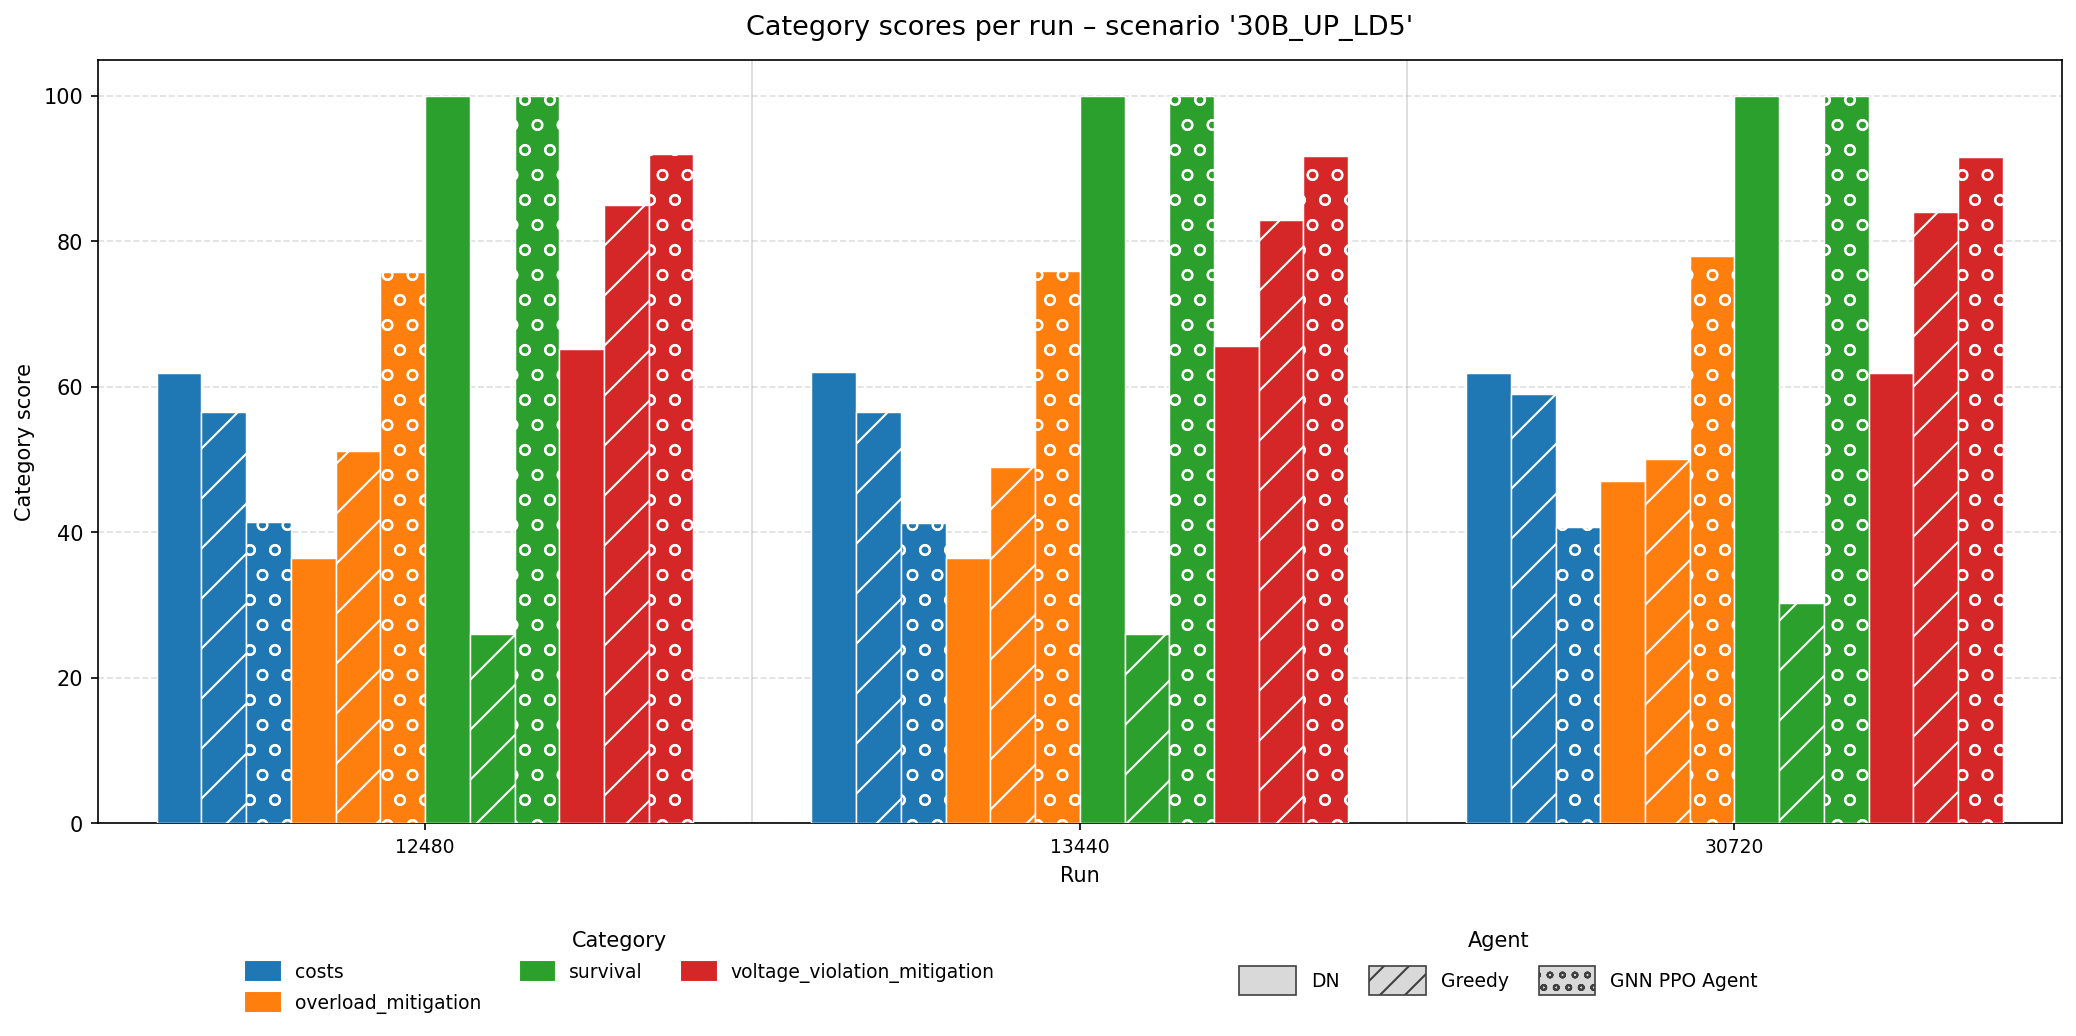
\includegraphics[width=0.93\textwidth]{images/experiments/scenario_scores/30B_UP_LD5.png}
        \caption{30-bus with increased power consumption in load 5}
        \label{fig:scenario-scores-30b-up-ld5}
    \end{subfigure}

    \vspace{0.2em}

    \begin{subfigure}[t]{1\textwidth}
        \centering
        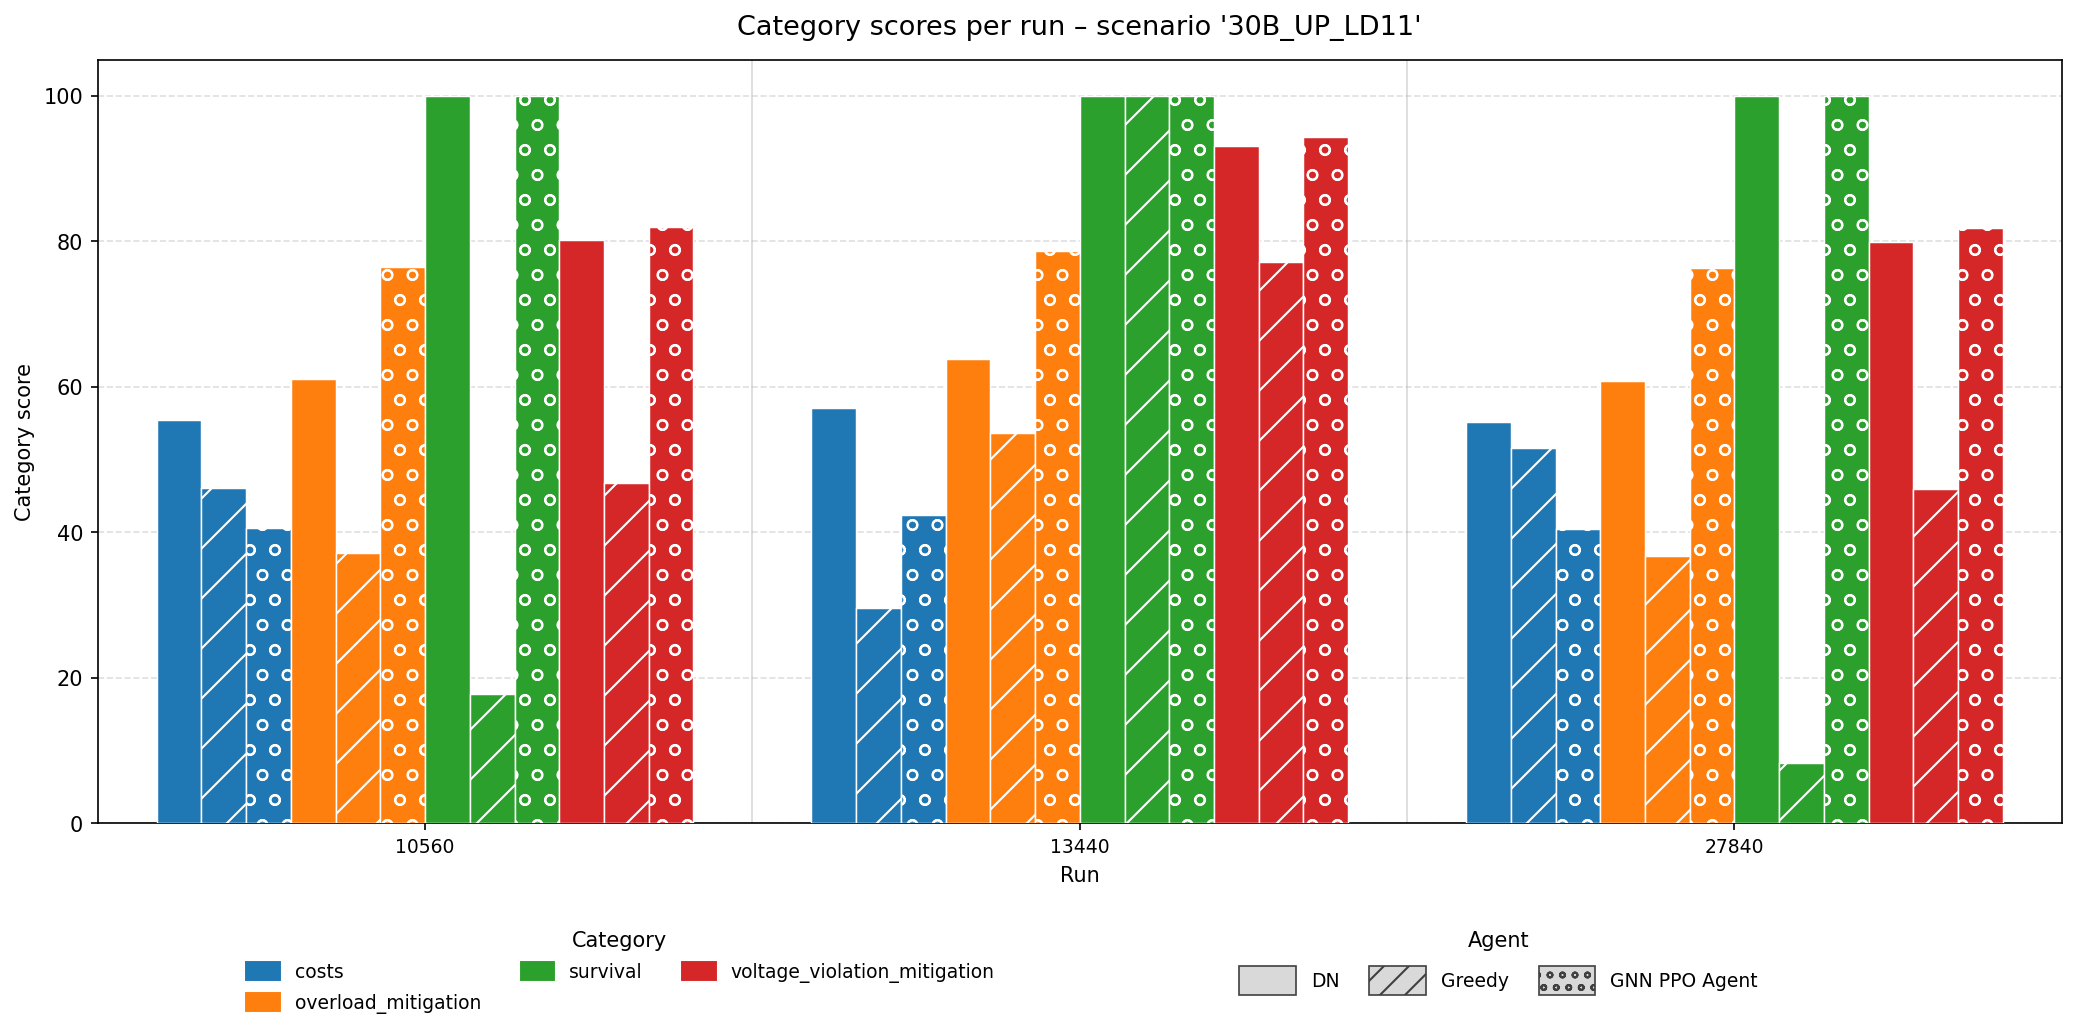
\includegraphics[width=0.93\textwidth]{images/experiments/scenario_scores/30B_UP_LD11.png}
        \caption{30-bus with increased power consumption in load 11}
        \label{fig:scenario-scores-30b-up-ld11}
    \end{subfigure}

    \caption{Score overview over the scenarios in the 30-bus grid where loads were modified}
    \label{fig:scenario-scores-30b-ld-scaled}
\end{figure}

\begin{figure}[htp]
    \centering
    \begin{subfigure}[t]{0.65\textwidth}
        \centering
        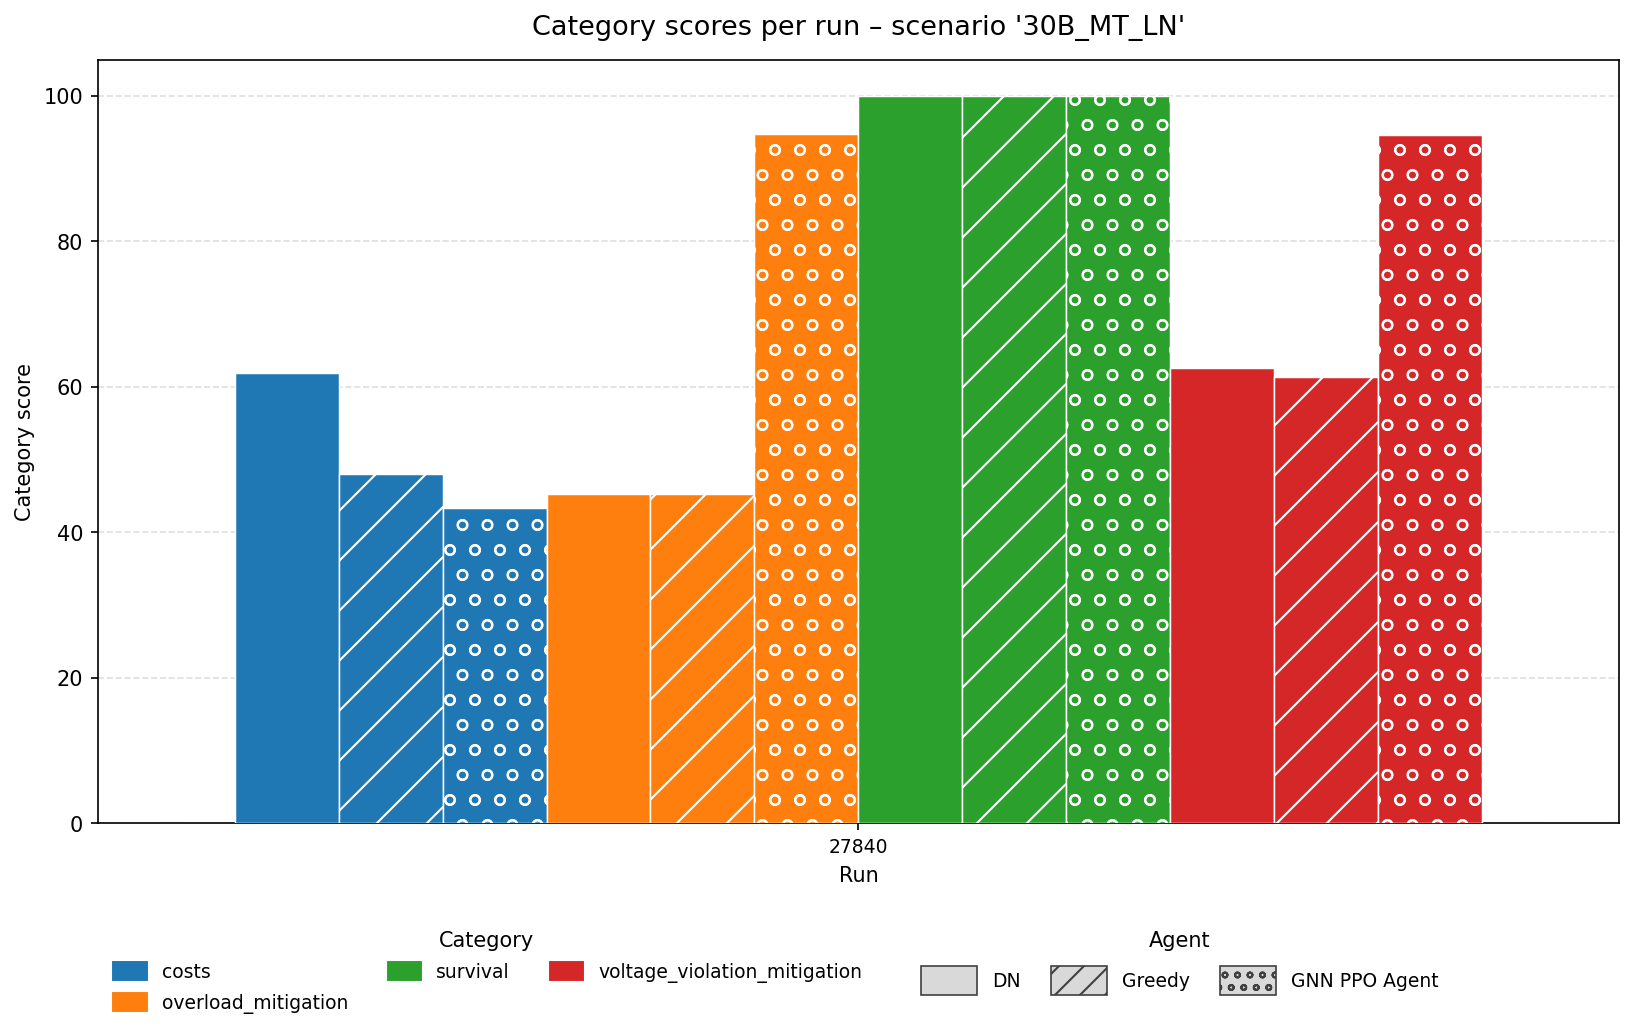
\includegraphics[width=\textwidth]{images/experiments/scenario_scores/30B_MT_LN.png}
        \caption{30-bus with maintenance in lines}
        \label{fig:scenario-scores-30b-mt-ln}
    \end{subfigure}
    \caption{Score overview over the scenarios where lines or generators had a maintenance event}
    \label{fig:scenario-scores-mnt}
\end{figure}

\begin{figure}[htp]\ContinuedFloat
    \centering
    \begin{subfigure}[t]{0.65\textwidth}
        \centering
        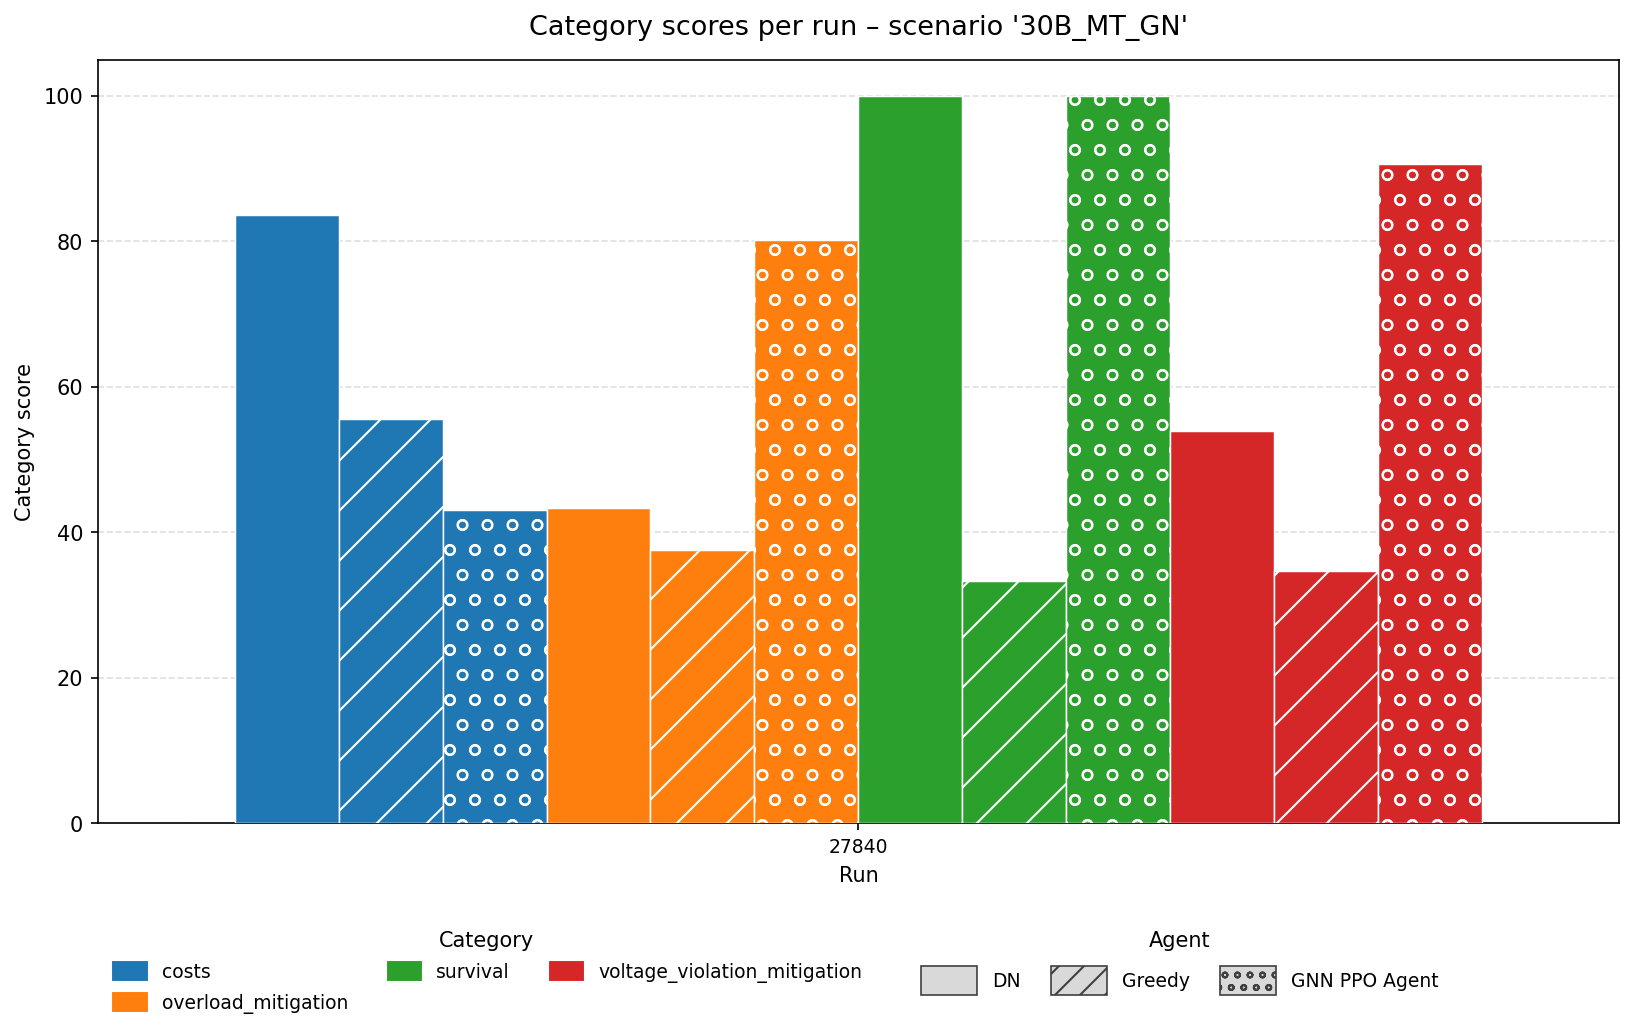
\includegraphics[width=\textwidth]{images/experiments/scenario_scores/30B_MT_GN.png}
        \caption{30-bus with maintenance in one generator}
        \label{fig:scenario-scores-30b-mt-gn}
    \end{subfigure}
    \caption{Score overview over the scenarios where lines or generators had a maintenance event (continued)}
\end{figure}

\begin{figure}[htp] % htp = hier (h), top (t), oder auf einer eigenen Seite (p).
    \centering
    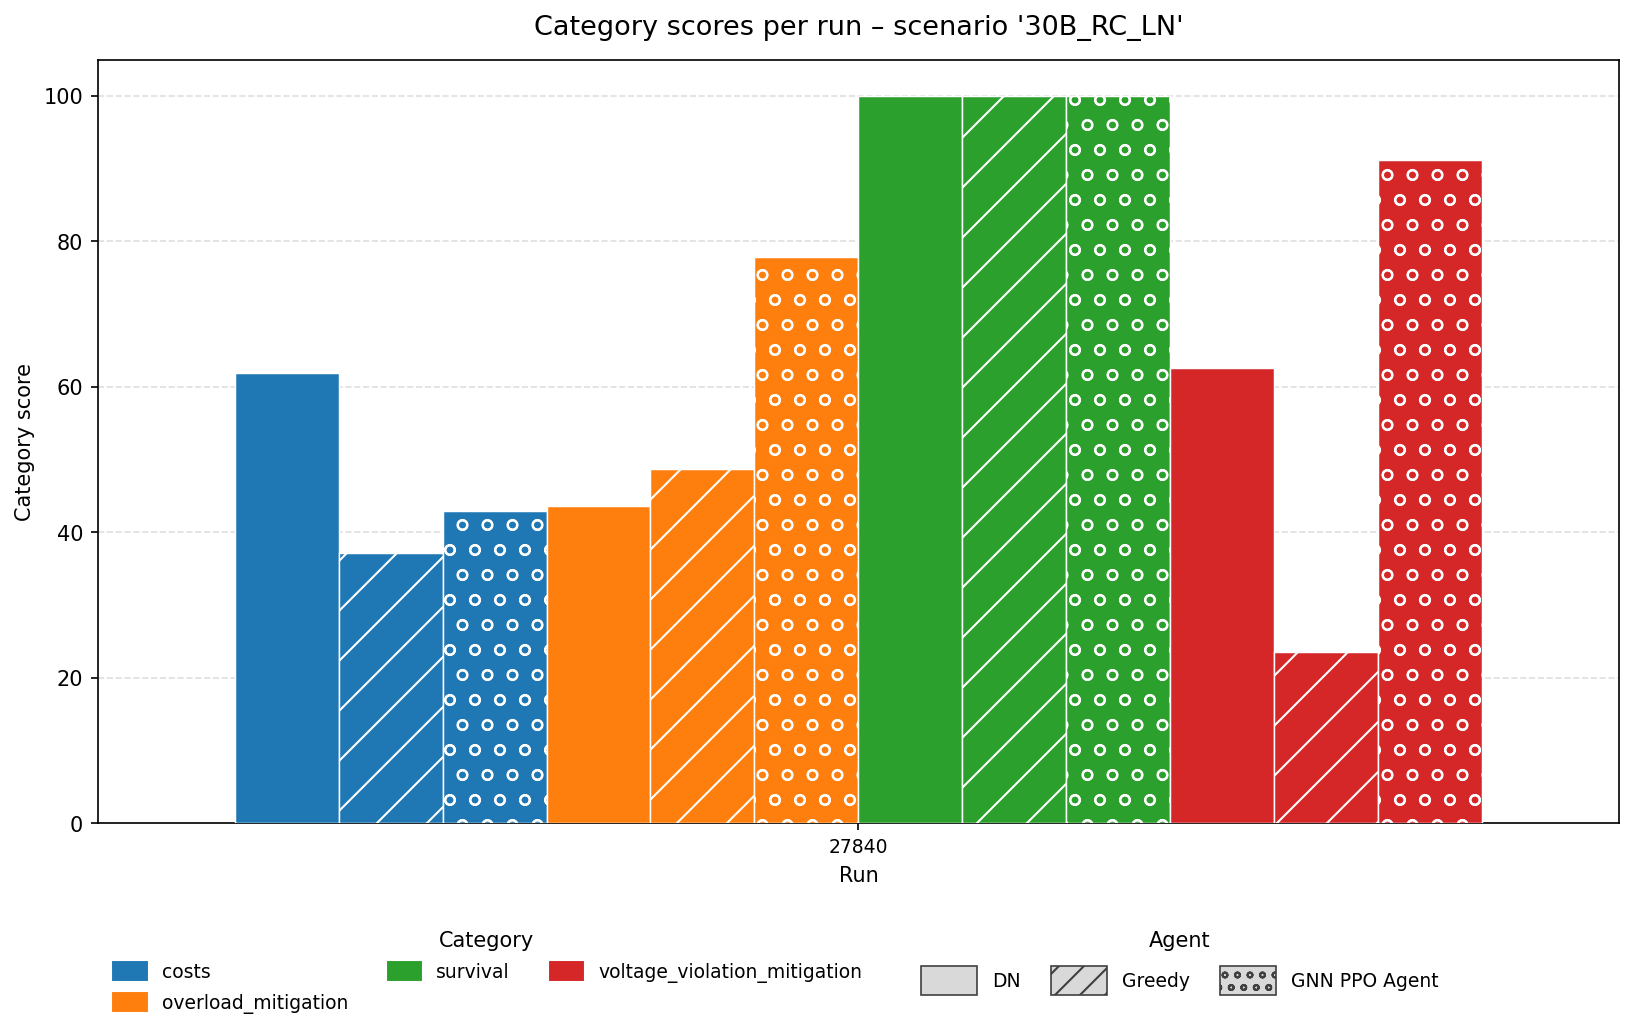
\includegraphics[width=0.7\textwidth]{images/experiments/scenario_scores/30B_RC_LN.png}
    \caption{Score overview over the scenario in the 30-bus power grid with lowered line capacity}
    \label{fig:scenario-scores-rc} 
\end{figure}

\FloatBarrier



\subsection{Stress Test Scenarios}
Figures \ref{fig:scenario-scores-gn-stress} to \ref{fig:scenario-scores-rc-stress} show the category scores achieved by the three agents on the individual scenarios composing the stress test experiments introduced in Section \ref{sec:exp-stress-test}, covering the lowest and highest stress levels of generator scaling, load scaling, and line capacity reduction. The second level of stress is already shown in the previous section.

\begin{figure}[htp] % htp = hier (h), top (t), oder auf einer eigenen Seite (p).
    \centering
    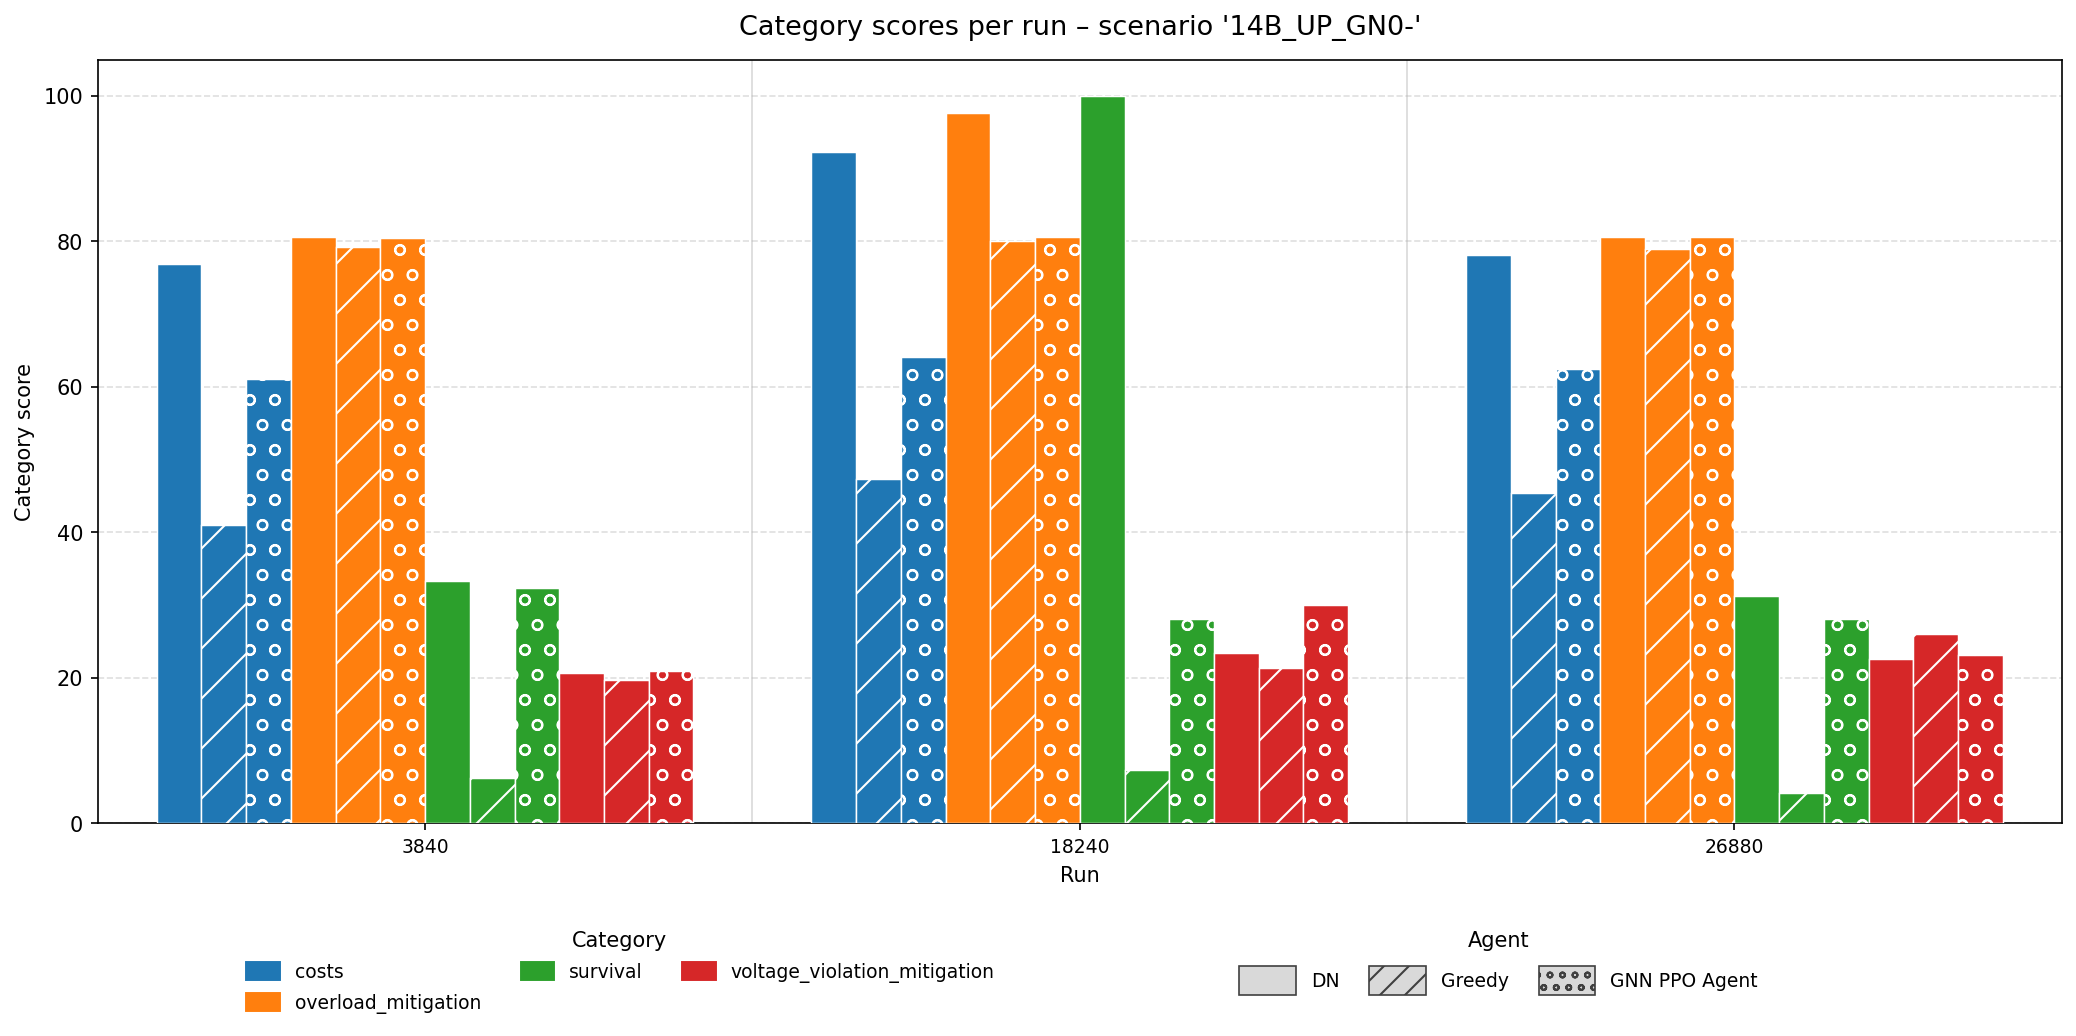
\includegraphics[width=0.95\textwidth]{images/experiments/scenario_scores/14B_UP_GN0-.png}
    \caption{Score overview over the scenario in the 14-bus power grid with lowest level of increased power generation in generator 0}
    \label{fig:scenario-scores-gn-stress} 
\end{figure}

\begin{figure}[htp]
    \centering

    \begin{subfigure}[t]{0.95\textwidth}
        \centering
        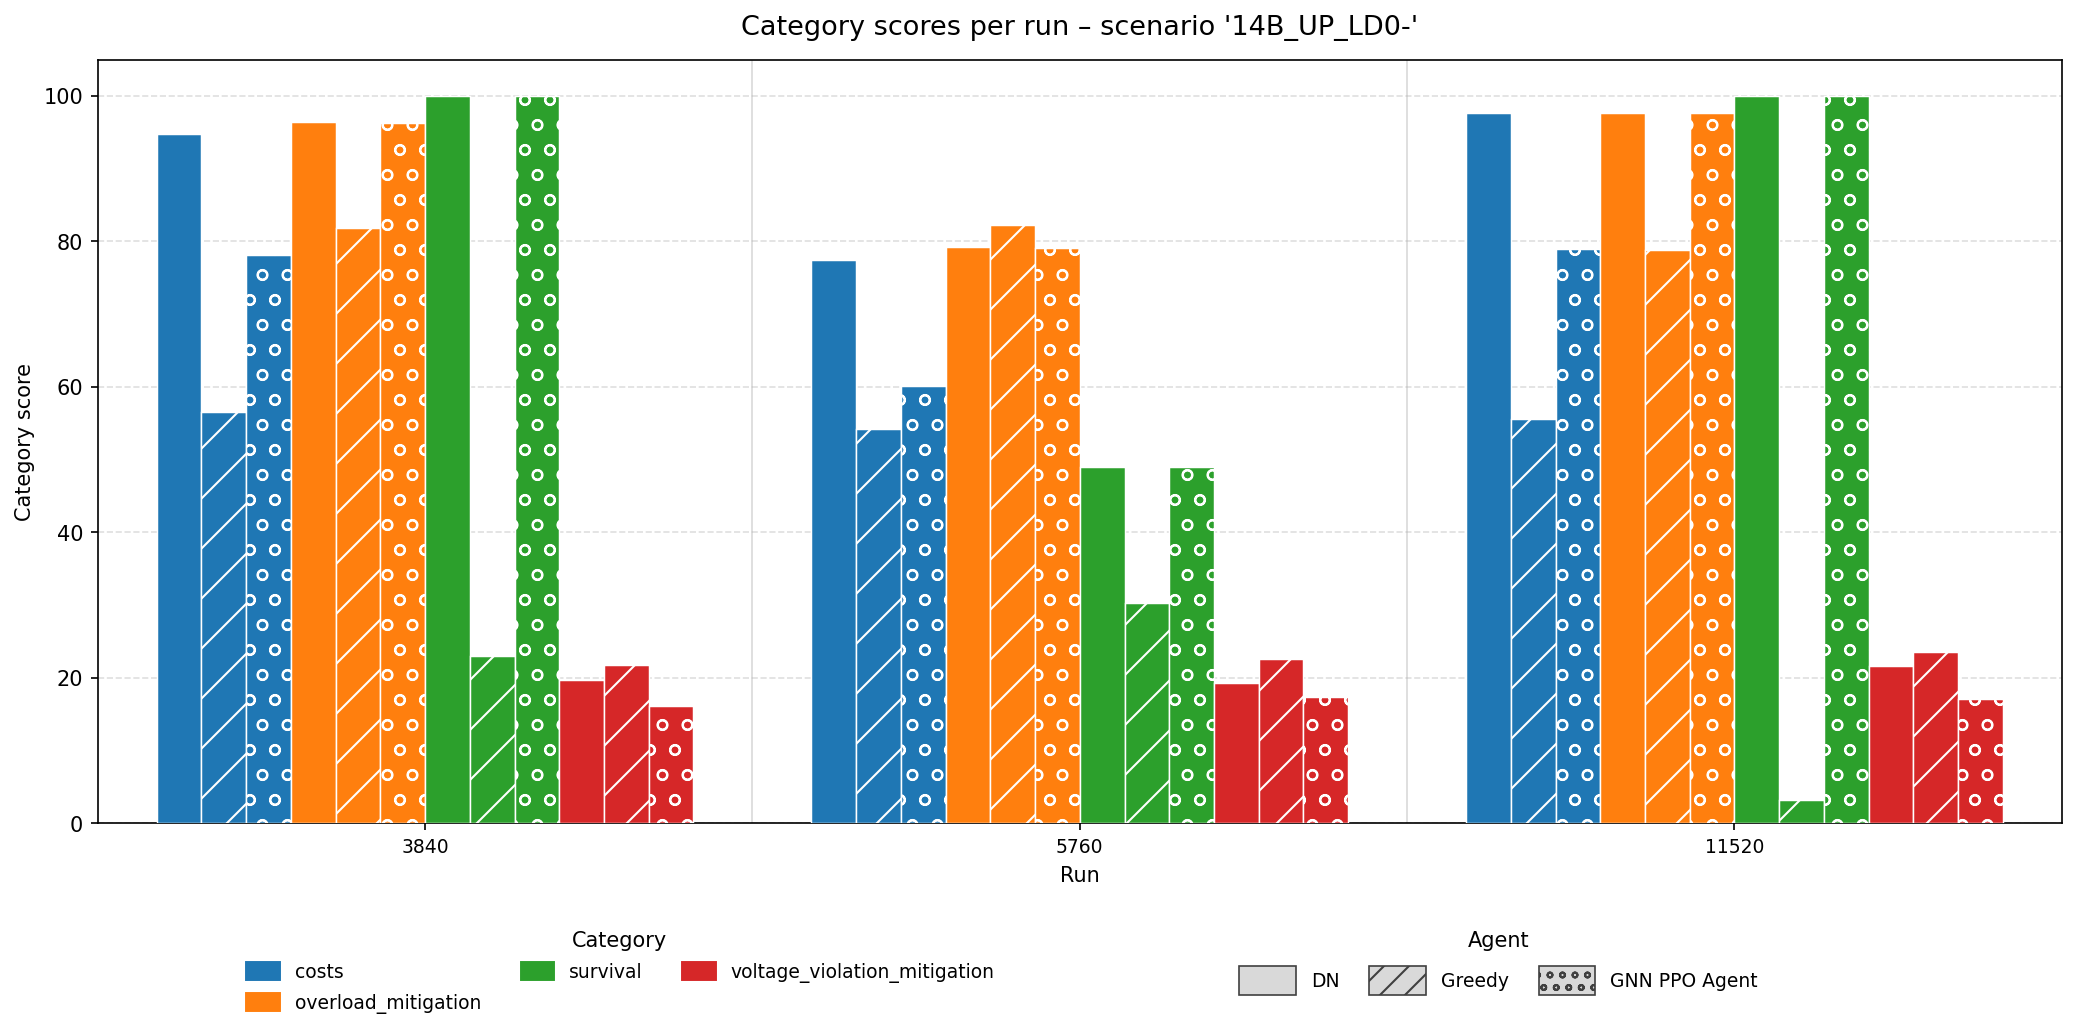
\includegraphics[width=\textwidth]{images/experiments/scenario_scores/14B_UP_LD0-.png}
        \caption{14-bus with lowest increased power consumption in load 0}
        \label{fig:scenario-scores-14b-up-ld0-low}
    \end{subfigure}

    \vspace{0.2em}

    \begin{subfigure}[t]{0.65\textwidth}
        \centering
        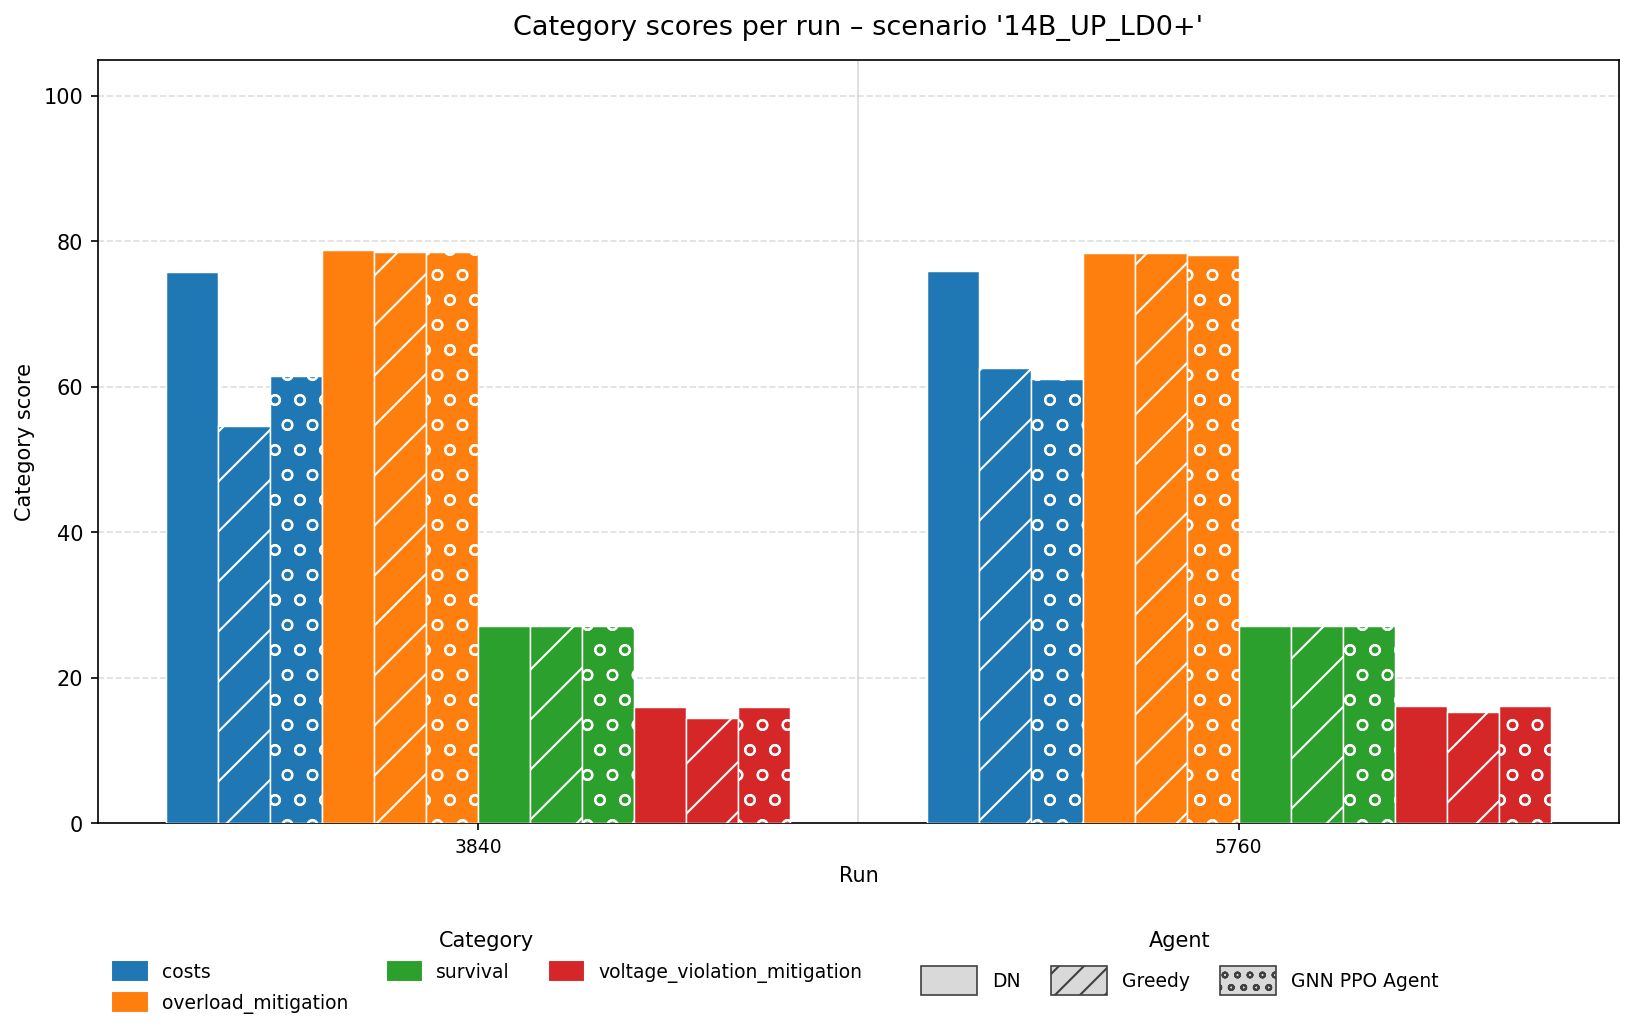
\includegraphics[width=\textwidth]{images/experiments/scenario_scores/14B_UP_LD0+.png}
        \caption{14-bus with highest increased power consumption in load 0}
        \label{fig:scenario-scores-14b-up-ld0-high}
    \end{subfigure}

    \caption{Score overview over the stress test scenario with different levels of load consumption scaling}
    \label{fig:scenario-scores-ld-stress}
\end{figure}

\begin{figure}[htp]
    \centering

    \begin{subfigure}[t]{0.65\textwidth}
        \centering
        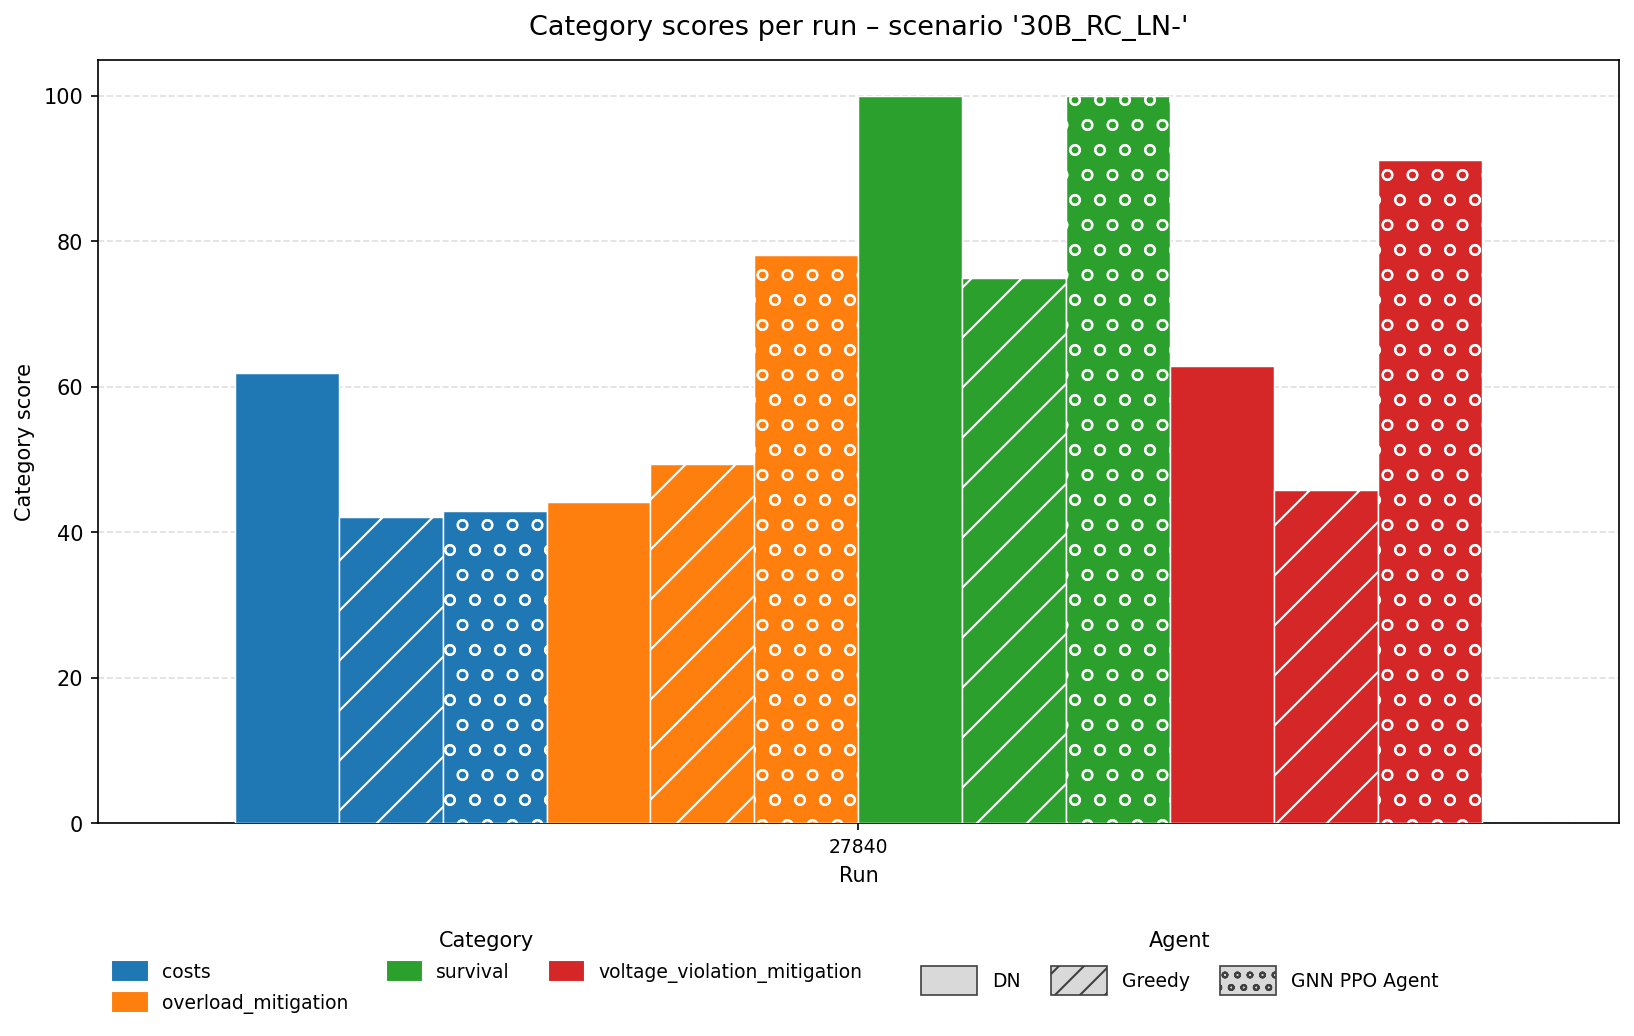
\includegraphics[width=\textwidth]{images/experiments/scenario_scores/30B_RC_LN-.png}
        \caption{30-bus with lowest reduced line capacity}
        \label{fig:scenario-scores-30b-rc-ln-low}
    \end{subfigure}

    \vspace{0.2em}

    \begin{subfigure}[t]{0.65\textwidth}
        \centering
        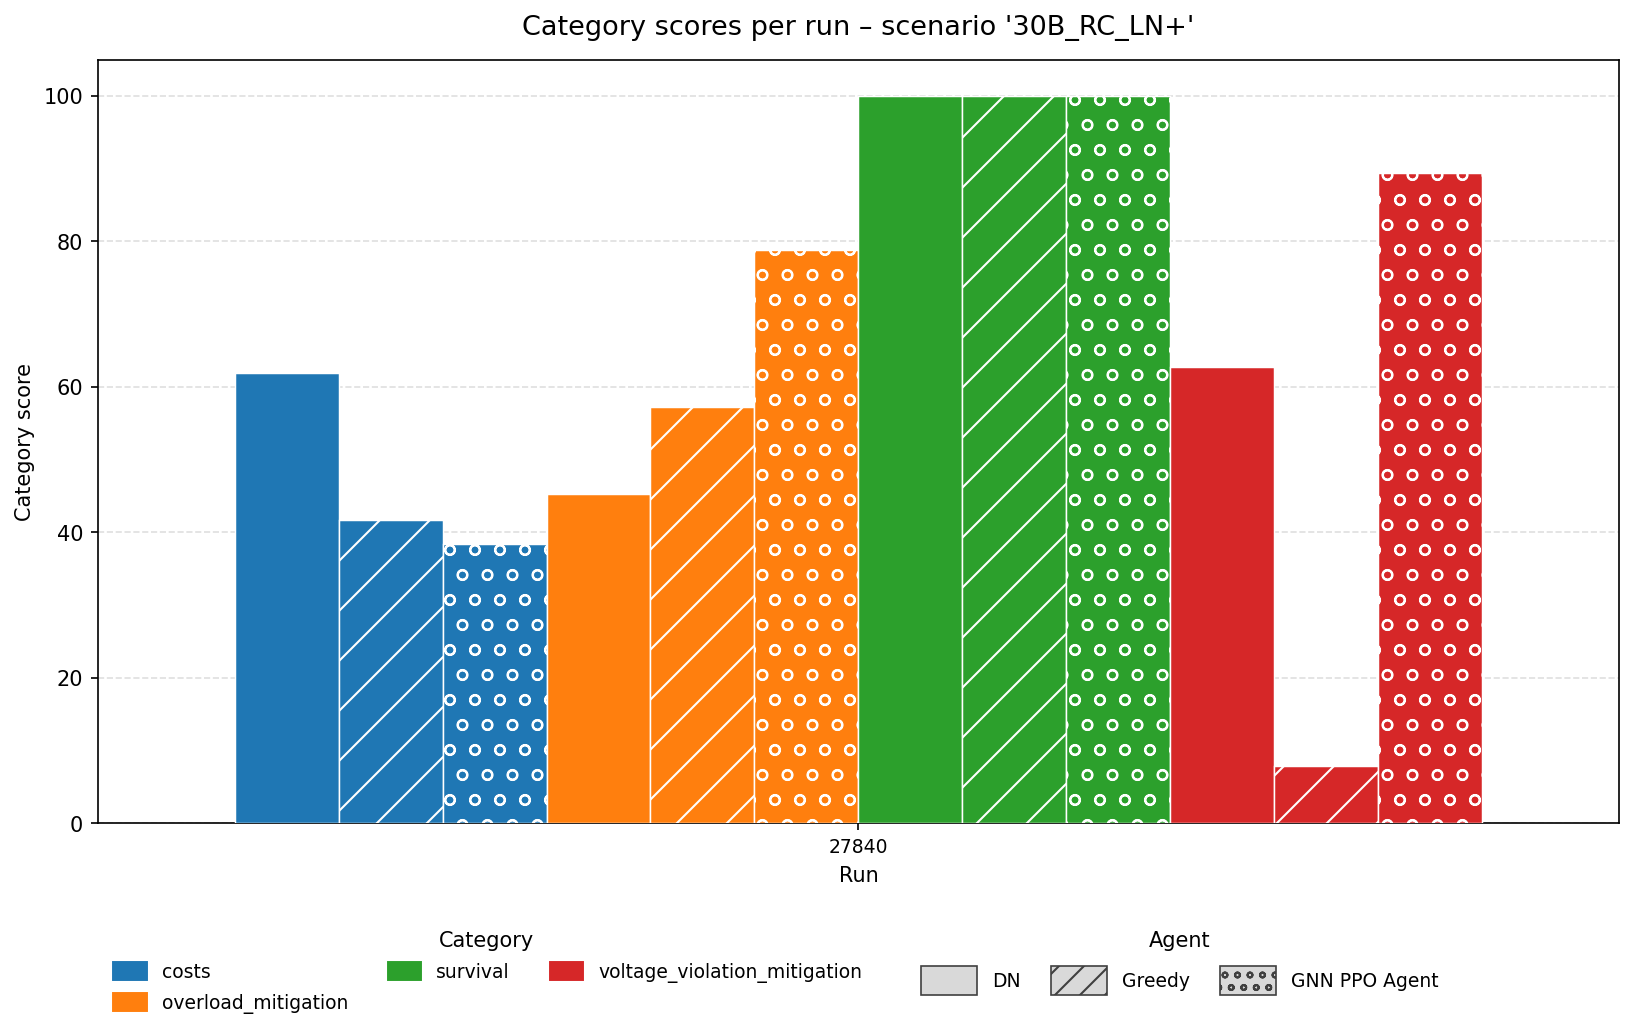
\includegraphics[width=\textwidth]{images/experiments/scenario_scores/30B_RC_LN+.png}
        \caption{30-bus with highest reduced line capacity}
        \label{fig:scenario-scores-30b-rc-ln-high}
    \end{subfigure}

    \caption{Score overview over the stress test scenario with different levels of line capacity scaling}
    \label{fig:scenario-scores-rc-stress}
\end{figure}

\FloatBarrier


\section{Case Study}\label{sec:exp-case-study}
Figure \ref{fig:grids-case-study} illustrates the partial grid topologies which result from the \ac{ppo} agent's substation-splitting actions in the three case studies discussed in Section \ref{ssec:case-studies}.

\begin{figure}[htp]
    \centering
    \begin{subfigure}[b]{0.48\textwidth}
        \centering
        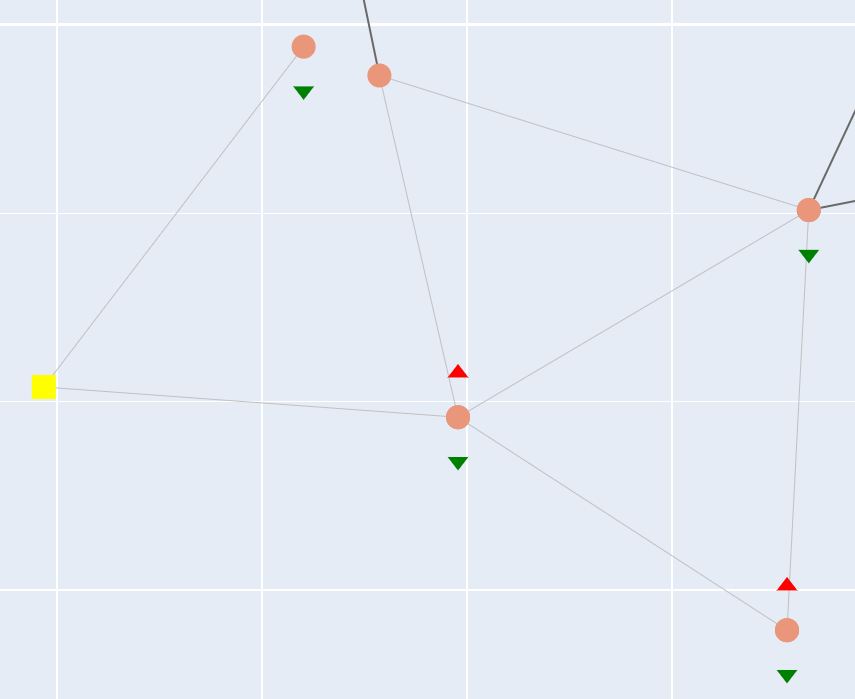
\includegraphics[width=\textwidth]{images/experiments/grids/case_study1.png}
        \caption{Partial power grid of case study 1, after the \ac{ppo} splitting action}
        \label{fig:grid-case-study1}
    \end{subfigure}
    \hfill
    \begin{subfigure}[b]{0.49\textwidth}
        \centering
        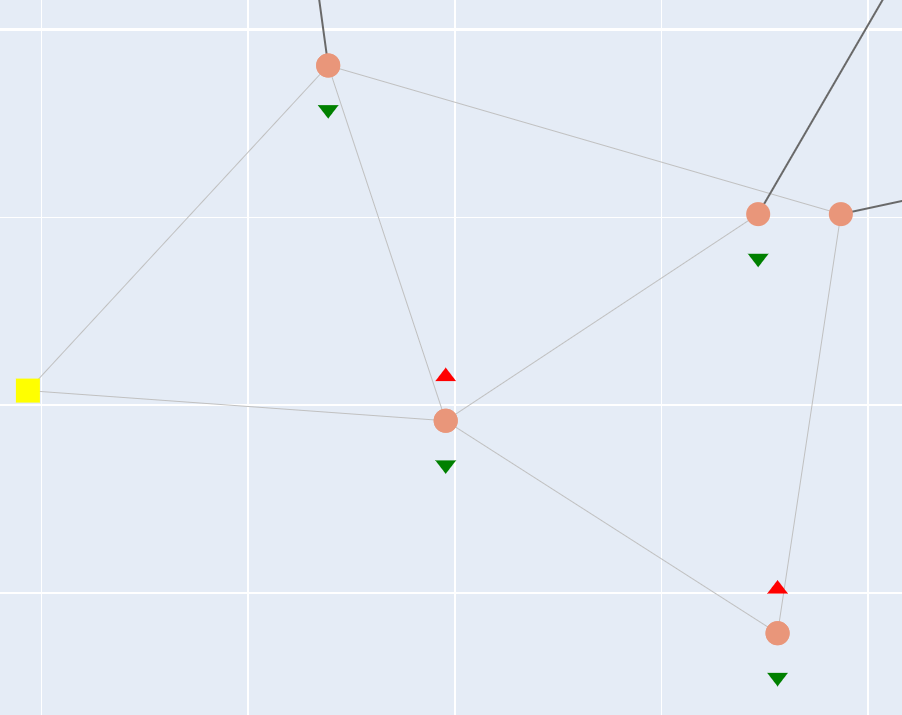
\includegraphics[width=\textwidth]{images/experiments/grids/case_study2.png}
        \caption{Partial power grid of case study 2, after the \ac{ppo} splitting action}
        \label{fig:grid-case-study2}
    \end{subfigure}

    \vspace{1em}

    \begin{subfigure}[b]{0.49\textwidth}
        \centering
        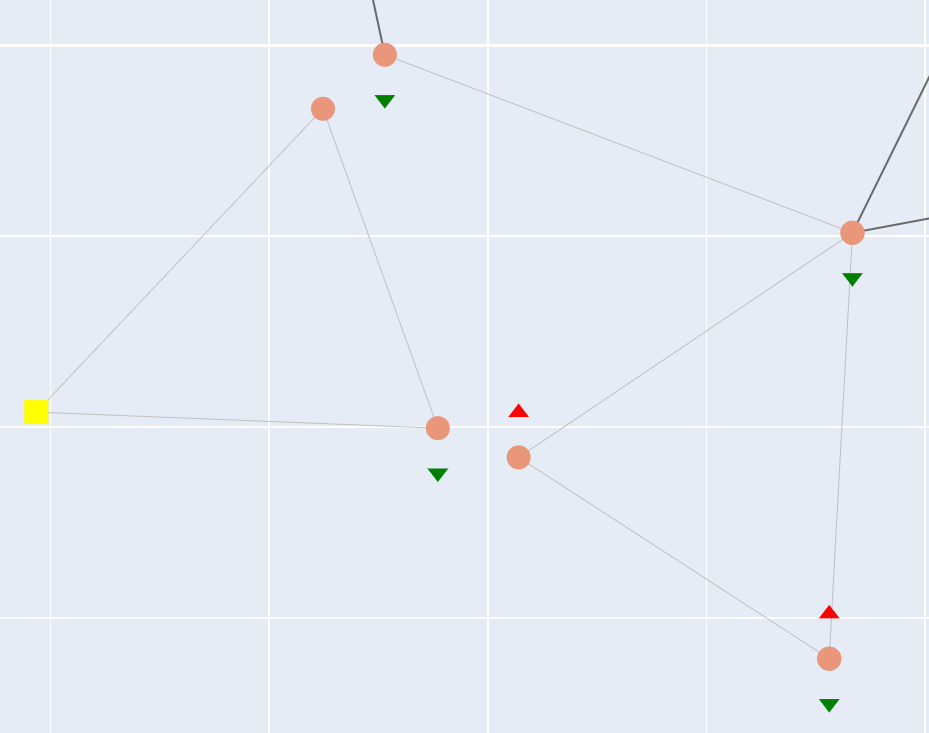
\includegraphics[width=\textwidth]{images/experiments/grids/case_study3.png}
        \caption{Partial power grid of case study 3, after the \ac{ppo} splitting actions}
        \label{fig:grid-case-study3}
    \end{subfigure}
    \caption{Power grids showing the actions made of the \ac{ppo} agent for the three case studies}
    \label{fig:grids-case-study}
\end{figure}

\FloatBarrier